%-----------------------------------------------------------------------------%
%Packages%
\documentclass[12pt, a4paper, titlepage]{article}
\usepackage{amsmath, amsfonts, listings, amssymb, mathtools, amsthm} %Mathematical Expressions package
\usepackage{mathtools}
\usepackage[usenames, dvipsnames]{color} %Color naming packages
\usepackage{geometry}
\usepackage{float}
\usepackage{verbatim} %for code
\usepackage[pdftex]{graphics}
\usepackage{hyperref}
\usepackage{cleveref}
\usepackage{tikz}
\usepackage{comment}
\usepackage[nottoc]{tocbibind}
%\usepackage[square]{natbib}
\usepackage{caption}
%\usepackage{subcaption}

\usetikzlibrary{arrows,shapes}

%Graphis Extensions
\DeclareGraphicsExtensions{.png, .jpg}
\parindent 0pt

% Predefined things such as commands, etc.

\newtheorem{defn}{Definition}[subsection]
\newtheorem{thm}{Theorem}[subsection]
\newtheorem{lemma}{Lemma}[subsection]
\newtheorem{corr}{Corrollary}[subsection]
\newtheorem*{remrk}{Remark}

\numberwithin{equation}{section}

\newcommand{\cover}{\bigtriangledown}
\newcommand{\sqex}[1]{[{#1}]}
\newcommand{\anex}[1]{\langle {#1} \rangle}
\newcommand{\lang}{\mathcal{L}}
\newcommand{\langRefine}{\lang_{\forall}}
\newcommand{\langActEx}{\lang_{\otimes}}
\newcommand{\langArbAct}{\lang_{\otimes\forall}}
\newcommand{\langProp}{\lang_0}

\newcommand{\AXK}{{\bf K}}
\newcommand{\AXAML}{${\bf AML_{\AXK}}$}
\newcommand{\AXRML}{${\bf RML_{\AXK}}$}
\newcommand{\AXAAML}{${\bf AAML_{\AXK}}$}

\newcommand{\axP}{{\bf P}}
\newcommand{\axK}{{\bf K}}
\newcommand{\axMP}{{\bf MP}}
\newcommand{\axNecK}{{\bf NecK}}
\newcommand{\axAN}{{\bf AN}}
\newcommand{\axAP}{{\bf AP}}
\newcommand{\axAC}{{\bf AC}}
\newcommand{\axAK}{{\bf AK}}
\newcommand{\axAU}{{\bf AU}}
\newcommand{\axNecA}{{\bf NecA}}
\newcommand{\axR}{{\bf R}}
\newcommand{\axRP}{{\bf RP}}
\newcommand{\axRK}{{\bf RK}}
\newcommand{\axRComm}{{\bf RComm}}
\newcommand{\axRDist}{{\bf RDist}}
\newcommand{\axNecR}{{\bf NecR}}

\newcommand{\kripkeClass}{\mathcal{K}}
\newcommand{\eventClass}{\mathcal{AM}}
\newcommand{\insaneClass}{\eventClass_{IN}}
\newcommand{\publicAnnClass}{\eventClass_{PA}}
\newcommand{\treeClass}{\eventClass_{TR}}
\newcommand{\forestClass}{\eventClass_{FOR}}

\newcommand{\FIXME}{{\bf FIXME}}
% Drawings of frames

\tikzstyle{vertex}=[circle,fill=black!25,minimum size=20pt,inner sep=0pt]
\tikzstyle{selected vertex} = [vertex, fill=red!24]
\tikzstyle{edge} = [draw,thick,->]
\tikzstyle{weight} = [font=\small]

%-----------------------------------------------------------------------------%
%Document%

\title{Languages for epistemic event model synthesis in multi-agent systems}
\author{Edwin Richard Yucheng Tay \\
University of Western Australia \\
email: taye03@student.uwa.edu.au }

\date{\today}

\begin{document}

\maketitle

\begin{abstract}

% A paper should begin with an insightful abstract, written in plain
% English and containing no references. It should state clearly the
% problem under consideration, the motivation for that problem, what you
% have achieved and how, and why your results are interesting.  All this
% in one paragraph too!

\end{abstract}

{\bf Keywords:} List, some, keywords, here.

\pagebreak

\tableofcontents

\chapter{Introduction} \label{chapter:intro}

Suppose Angeline and Ben are two share traders who fervently watch the stock market. They
are particularly concerned about the fate of company ABC and are waiting for news on whether ABC is
doing well or poorly. In the middle of their stock market vigil, Angeline is given a letter that says
ABC has done particularly well. Ben sees her open the letter and read its contents, but he does not
know what the letter is about.\\
\\
Our interest in Angeline and Ben's predicament centres mainly around their knowledge of company ABC.
We might ask questions, such as
\begin{itemize}
	\item What can we say about Angeline and Ben's knowledge before the letter arrives?
	\item What could we say about their knowledge after the letter's arrival?
	\item What about Ben in particular --- what does he know, and what does he not know or is unsure about?
\end{itemize}
An epistemic model of this situation concerns itself with the information regarding company ABC, and
what each of our agents knows or believes about the situation.\\
\\
If we wish to formally model Angeline and Ben's stock situation, we must consider how we can model
\begin{enumerate}
	\item The facts Angeline and Ben know or believe before Angeline obtained the letter
	\item The change in belief or knowledge described by Angeline's letter and Ben's observations; and
	\item The updated facts Angeline and Ben know or believe after the letter has been opened
\end{enumerate}

Epistemic modal logic is particularly concerned with modelling item one --- the study of knowledge,
belief and the interplays of uncertainty.
For example, an epistemic model can model the possibilities that Angeline and Ben believe --- a
possibility where the company ABC has done well, and a possibility where the company ABC is
performing poorly.\\
\\
The epistemic models of the situation prior to Angeline seeing her letter further model how both Angeline
and Ben do not know whether company ABC is doing poorly, and that they also do not know whether
that company ABC is doing well.
However they cannot tell the difference between either of these possibilities.\\
\\
Modelling epistemic situations, in accordance with axiomatic schemes that
formally model knowledge, is a well-studied field.
The work in this area has been used in financial trading and games to reason about the knowledge
that agents in these systems have, as well as model checking and automated theorem proving.
Automated reasoning about knowledge, and maintaining it in a consistent state are two important 
Epistemic modal logic thus finds its uses when logical deductions about knowledge and belief must be
made, as well as proving that an agent knows or believes exactly some set of propositions at a
particular time step.\\
\\
This work is particularly concerned with how we model the letter that Angeline receives and Ben
indirectly infers from Angeline's reading of it.
Furthermore, we are interested in the new knowledge and beliefs that Angeline and Ben possess after the update.
What does Ben know after Angeline has read the letter?
How can we model the information in the letter so that Angeline is informed of company ABC's success,
and Ben is not?\\
\\
These questions that are related to items two and three --- changes in knowledge, and how we can
model the results of changes.
Work in this area is relatively new, and dynamic epistemic modal logic is of particular concern
within this paper.
In particular, being able to reason about the effects of changes, and to prove their properties and
effects is desirable.\\
\\
One method of representing updates is the concept of action models, as
introduced by Baltag, Moss and Solecki \cite{baltag1998lpa}.
A large body of work has been centred on specifying action models and reasoning
about their properties.
Our work looks at a different aspect of action models --- how to compose smaller action models
into larger ones under the constraints of a meaningful framework.\\
\\
In the case of Angeline and Ben, we might consider composition as a taking a series of sentences
regarding the performance of company ABC, such as ``Angeline knows that ABC is doing well", ``Angeline
believes that Ben believes ABC is doing poorly" or simply ``ABC is doing poorly".
Those sentences are composed together into a meaningful and useful letter that Angeline and Ben can
understand regarding the performance of company ABC (e.g. ``Angeline knows that ABC is doing well
and Angeline believes that Ben believes ABC is doing poorly").
These letters might in turn be sent to Angeline and Ben in bulk, as one large update to their knowledge
about ABC.\\
\\
Composition unifies some approaches to representing changes in knowledge with action models, namely
around representing action models as formulae and providing a language for updating action models.
Updates (the letters in the ABC example) can be written in terms of atomic updates (the sentences)
and operations which compose them together.
We specify a meaningful language that constructs larger action models out of atomic updates, and
show that it can effectively construct all updates.\\
\\
This work will document the different languages and the operations used in them to construct
different epistemic updates.
We will show a complementary work to Hales' \cite{hales13synthesis} work that constructs updates in the weakest modal logic,
$\AXK$, which is far removed from epistemic modal logic.
We then change axiom systems to a modal logic that reflects typical properties of knowledge,
$\AXKFF$, and show how we can construct updates in that logic.\\
\\
The rest of this paper is arranged as follows
\begin{itemize}
	\item Chapter \ref{lit_survey} gives an overview of the state of the art of epistemic modal logic
		and clearly outlines what problems the work in this thesis aims to solve
	\item Chapter \ref{chapter:prelim} gives the technical definitions, lemmas and theorems
		established in previous works
	\item Chapter \ref{chapter:Multiagent} shows results that compliment Hales' work in
		\cite{hales13synthesis}, particularly in constructing action models for epistemic goal
		achievement in $\AXK$
	\item Chapter \ref{chapter:k45} shows our results in constructing action models for epistemic goal
		achievement in $\AXKFF$, which is an axiom system that more closely resembles epistemic modal
		logic
\end{itemize}

\chapter{Literature survey} \label{lit_survey}

Within this chapter we consider the relevant writings and logics to describe
the epistemic state and how we can change and informatively update the epistemic
state.
We will explore how we can model static situations and
different informative updates.
We will note what has not been explored in the fields and compare frameworks'
differing approaches and strengths.\\
\\
To explore the techniques used to model information and the change of information, we introduce an
example of a game of information.
Consider a game being played between two friends (agents), Angeline $(A)$
and Ben $(B)$.
The game involves flipping a coin, hiding the result from both $A$ and $B$ and
having both of them guess whether the coin is Heads $(H)$ or the coin is Tails
$(T)$.
The game is refereed by a mutually trusted (and usually impartial) friend, Carol
$(C)$ who knows if the coin is $H$ or $T$.\\
\\
$A$ and $B$ know that either $H$ is true or $T$ is true.
They also know that $H$ and $T$ cannot both occur simultaneously together.
An agent's knowledge (which is inclusive of, but not limited to the previous
statements) is called the epistemic state.
Furthermore, there are two possibilities for the coin's outcome: that it is $H$
or $T$.
Neither $A$ or $B$ as they are can distinguish between them; that is, they are
uncertain which of the outcomes is true.
Agent uncertainty in this multi-agent system is another aspect we must attempt
to capture.

\section{Epistemic modal logic}\label{survey_epistemic_modal_logic}
In our coin-flipping game, we can make the following observations.
\begin{itemize}
	\item $A$ considers $H$ to be possible, as well as $T$ to be possible
	\item $B$ also considers $H$ to be possible, and also considers $T$ to be possible
\end{itemize}
We claim that there are two possible worlds that differ in one way ---
in one of these worlds, $H$ is true, and in the other world $T$ is true.
Furthermore, these worlds are the same from $A$ and $B$'s perspectives.
$A$ would not be able to distinguish the world where $H$ was true from either of
the world where $H$ was true or the world where $T$ was true, since she cannot
see the coin.\\
\\
We can represent this uncertainty between what world is true as relations
between worlds.
In this case, let $W = \{ \eta, \tau\}$ be our set of possible worlds, where $H$ is true
at $\eta$ and $T$ is true at $\tau$.
Let $R_A = R_B = \{(\tau,\tau), (\tau,\eta), (\eta, \tau), (\eta,\eta)\}$ be
binary relations on $W$ representing indistinguishability between two possible
worlds.
We call these relations ``accessibility relations"; we say if one world is
indistinguishable from another, then they can access each other.
Lastly, let $V$ be a valuation function that maps a formula to the set of worlds
where that formula is true, so $V(H) = \{\eta\}$ and $V(T) = \{\tau\}$.\\
\\

\begin{defn}
	The tuple
	\[
		M = (W, R = R_A \cup R_B, V)
	\]
	is an epistemic model of our game of heads and tails.
\end{defn}

These definitions, as well as a more formal, in-depth treatment of modal logic and
the possible worlds model, is given in reference texts by Blackburn, de Rijke and Venema \cite{blackburn2002modal},
as well as van Ditmarsch, van der Hoek and Kooi \cite{hoek2008dynamic}.
We also redefine models formally in Definition \ref{model}.

We can represent this model graphically as shown in Figure \ref{htkripkefigure},
where our possible worlds $(W)$ are nodes and our binary relations $(R$) are edges in the
graph.

\begin{figure}[ht!]
\centering
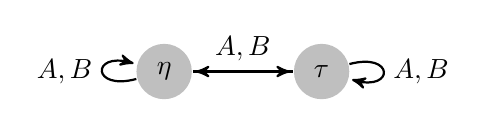
\begin{tikzpicture}[->,>=stealth',shorten >=1pt,auto,node distance=2cm,
      thick]

    \node[vertex] (1) {$\eta$};
    \node[vertex] (2) [right of=1] {$\tau$};
    \path[edge]
          (1) edge node {$A,B$} (2)
              edge [loop left] node {$A,B$} (1)
          (2) edge node {} (1)
              edge [loop right] node {$A,B$} (2);
\end{tikzpicture}
\caption[Possible worlds game of heads and tails.]{A graph representation of our game of heads and tails.}\label{htkripkefigure}
\end{figure}

The possible worlds models form a semantics allowing us to construct meaningful
models that reflect an epistemic state.
It is the semantics and models that allow us to reason about relations between the possible worlds in
an internal sense, from $A$ and $B$'s perspectives \cite{blackburn2002modal}.
We can define an operator to formally represent the modality of ``knowing"
a proposition or formula to be true.

\begin{defn}
	The operator $\Box_a H$ stands for ``Agent $a$ knows $H$ is true".
	$\Box_a \phi$ is true at a possible world $w$ if for all accessibility relations $(w,
	w')$, $\phi$ is true.
\end{defn}

We also define the dual operator of knowing, which is to consider something
possible.

\begin{defn}
	The operator $\Diamond_a T$ stands for ``Agent $a$ considers $T$ to be possible".
	$\Diamond_a \phi$ is true at a possible world $w$ if there is one
	accessibility relation $(w,w')$ such that $\phi$ is true at $w'$.
\end{defn}

Notice that we can define $\Diamond$ in terms of $\Box$, where $\Diamond_a
\phi \iff \neg \Box_a \neg \phi$.\\
\\
The definitions for $\Box_a$ and $\Diamond_a$ are given a more formal treatment in
Fagan et. al in \cite{fagin1995reasoning} and van der Hoek, Kooi and Ditsmarsch in
\cite{hoek2008dynamic}.
Both definitions are formally re-defined in Definition \ref{modalLogic}.\\
\\
We will omit the name of the agent for operators $\Box_a$ and $\Diamond_a$ when we
discuss a single-agent case, as follows.
We now show, without proof, four axioms that must hold for our modality of
knowledge.

\begin{propn}
	The following are true at any world of an epistemic model
	\cite{hoek2008dynamic}.
	\begin{enumerate}
		\item $\Box (\phi \implies \theta) \implies (\Box \phi \implies \Box
				\theta)$, known as {\bf K}
		\item $\Box \phi \implies \phi$, known as {\bf T}
		\item $\Box \phi \implies \Box \Box \phi$, known as {\bf 4}
		\item $\neg \Box \phi \implies \Box (\neg \Box \phi))$, known as {\bf 5}
	\end{enumerate}
\end{propn}

In order to satisfy these conditions, binary relations between possible worlds
in our epistemic models become equivalence relations.\\
\\
Also, if we replaced {\bf T} with an axiom {\bf D} which states $\Box \phi
\implies \Diamond \phi$, then we can model doxastic models of belief, instead of
epistemic models of knowledge.\\
\\
We can now make formal reasonings, such as deciding that $\Box_A H$ and $\Box_A
T$ are both false.
We note that $\Box_B (H \lor T)$ is true and $\Box_A \Box_B (H \lor T)$ is
true.\\
\\
{\bf K}, {\bf T}, {\bf 4} and {\bf 5} allow us to model epistemic state and
uncertainty in our game of heads and tails.
We have defined on our models that allows us to make formal reasonings and
decide if formulae are true at possible worlds.\\
\\
But what if their friend, $C$, announces ``The coin is Heads up"?
As they are, our epistemic models cannot describe the change in knowledge that
$C$'s announcement will entail.
Furthermore, we have no formal process to say how the situation has changed.\\
\\
This deficiency raises the following questions:
\begin{itemize}
	\item How do we describe this change in a formal manner?
	\item What reasoning can we make about the state of information after this
	change?
	\item Is there an operation that allows us to change the state of information
	from the pre-change state to the post-change state?
\end{itemize}

\section{Public announcement logic}\label{pal}
To model the announcement of facts and information, we turn to the use of public
announcement logic.
Public announcements are announcements to multiple agents of facts.
They are a kind of informative update --- perhaps the most basic kind.\\
\\
Public announcement logic was first proposed independently by both Plaza and
Gerbrandy and Groeneveld \cite{plaza2007public,gelbrandy1997reasoning}.
They were later augmented by the work of Baltag, Moss and Solecki through the
addition of common knowledge \cite{baltag1998lpa}.
Public announcements are informational updates of true facts that change the
knowledge state amongst multiple agents.\\
\\
In the context of our card game, let us consider if our external trusted party
$C$ publicly announces to $A$ and $B$ that $H$ is true.
We will demonstrate the execution of that update upon our model in Figure
\ref{pakripkefigure}.

\begin{figure}[ht!]
\centering
\begin{subfigure}[b]{.45\textwidth}
\centering
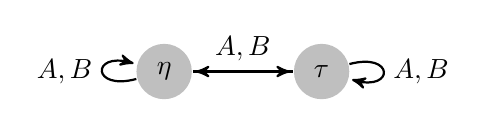
\begin{tikzpicture}[->,>=stealth',shorten >=1pt,auto,node distance=2cm,
      thick]
    \node[vertex] (1) {$\eta$};
    \node[vertex] (2) [right of=1] {$\tau$};
    \path[edge]
          (1) edge node {$A,B$} (2)
              edge [loop left] node {$A,B$} (1)
          (2) edge node {} (1)
              edge [loop right] node {$A,B$} (2);
\end{tikzpicture}
\caption{Our model before $H$ is announced to be true.}
\label{beforefigure}
\end{subfigure}
~
\begin{subfigure}[b]{.45\textwidth}
\centering
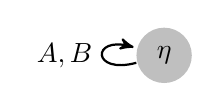
\begin{tikzpicture}[->,>=stealth',shorten >=1pt,auto,node distance=2cm,
      thick]

    \node[vertex] (1) {$\eta$};
    \path[edge]
          (1) edge [loop left] node {$A,B$} (1);
\end{tikzpicture}
\caption{Our model after $H$ is announced to be true.}
\label{afterfigure}
\end{subfigure}
\caption[Public announcement: before and after]{The differences before and after the public announcements of $H$ to $A$ and
	$B$.}
\label{pakripkefigure}
\end{figure}

Public announcements capture changes in information, such as $C$ saying to
$A$ and $B$ that the coin is $H$.
Another possible update is $A$ being allowed to see the coin's state, and
telling $B$ ``I guess you didn't know that the coin is actually heads up".\\
\\
These changes can be successful or unsuccessful, depending on whether the fact
that was announced is true after its announcement.
For example, if $A$ makes the (truthful) announcement that $H$, then this
announcement is successful since $H$ will be true after the announcement.\\
\\
Conversely, an announcement from $A$ to $B$ that ``I know that you {\em don't} know $H$
is true, but the coin is actually $H$".
We can write this as the announcement of the formula $H \land \neg \Box_B H$.
We can again refer to Figure \ref{pakripkefigure} to graphically show the models
before (Figure \ref{beforefigure}) and after (Figure \ref{afterfigure}) the update.
This update is interesting in that its announcement causes itself to be false.\\
\\
When $A$ publicly announces that the coin is $H$ and that $B$ does not know that
the coin is $H$ her announcement is now false, since $B$ now knows that $H$
actually is true.
Examining Figure \ref{afterfigure}, we can see that $H \land \neg \Box_B H$ is
untrue after its announcement in Figure \ref{beforefigure}.
This is an example of an unsuccessful public announcement.\\
\\
By using public announcement logic we can describe these announcements of
information.
We have a framework to describe and change the state of information amongst our
agents before and after announcements of facts.
Public announcement logic will allow us to model $C$ telling $A$ and $B$ in a
public fashion that $H$ is true.
This scales to modelling broadcasts in multi-agent systems, and allowing us to
update our models of the epistemic state of agents in such mass, public communications.\\
\\
In terms of dynamic epistemic logic, however, there could be many more kinds of
updates that we have yet to consider.
Re-examining our game of heads and tails yields scenarios that we cannot
describe:
\begin{itemize}
	\item What about $A$ cheating and learning $H$ or $T$ without $B$'s knowledge?
	\item What if $C$ was to whisper (in front of $B$) whether the coin was $H$
	or $T$?
\end{itemize}
These are things public announcement logic cannot describe, and our inability to
model them raises more questions:
\begin{itemize}
	\item what other kinds of epistemic (or informative) updates exist?
	\item how can we describe other epistemic updates in a sensible manner?
	\item what kind of an execution is required for a more nontrivial update?
\end{itemize}

\section{Epistemic actions and action models} \label{estAct}
We can now successfully capture the simple act of announcing a fact.
However, in public announcements, we cannot capture certain updates to the
epistemic state, such as
\begin{itemize} 
  \item $C$ whispers to $A$ that $H$ is true and $B$ sees her whisper
  \item $C$ whispers to $A$ that $H$ is true without $B$ seeing
  \item $B$ suspects $A$ of cheating, but he isn't sure if she's cheated
\end{itemize}
Let us aim to generalise the ideas behind public announcements to capture other
informative updates.\\
\\
We will now constrain our agents' behaviours to only being able to accept facts.
They will not worry about changing facts, and if facts do change we will take it
as something that causes our agents knowledge systems to simply crash.\\
\\
We will examine two contrasting approaches to model these epistemic updates.
Our investigation will show the main differences in terms of what the frameworks
can describe and how we can use them to reason about updates.
\subsection{Epistemic relational actions} \label{epi_acts}
van Ditmarsch approaches epistemic actions from a syntactical point of view,
aiming to create a language to specify actions in.
His work in constructing an epistemic action syntax extends some of the
syntax of established languages such as propositional dynamic
logic \cite{ditmarsch99knowledge,ditmarsch2002dga}.\\
\\
van Ditmarsch provides operations to construct dynamic epistemic formulae, and
further extends the language with dynamic or action-oriented constructs.
These include the ability to test a proposition, to update a group of agents'
knowledge and to make a non-deterministic choice between actions.
Thus, van Ditmarsch presents a way to describe complex actions, and indeed we can
express and describe all the actions we've discussed in the previous sections.
We can formally describe actions such as cheating, or a private
announcement to $B$ that $H$ is true that's seen by $A$.\\
\\
However, reasoning about epistemic actions in their current form is difficult.
Indeed, the interpretations of an epistemic action are non-trivial to
understand.
Moreover, van Ditmarsch, van der Hoek and Kooi present problems with
representing complex uncertainties with van Ditmarsch's epistemic actions that make it difficult
to reason about what $A$ and $B$ know after an action takes place.\\
\\
In the next section, we review a different framework to model epistemic updates
which can describe as many updates as van Ditmarsch's language.
This framework resolves the issues with van Ditmarsch's epistemic actions and
has uncertainty about actions naturally encoded within it.
\subsection{Epistemic action models} \label{act_mods}
As an alternative to approaching epistemic actions syntactically, Baltag, Moss
and Solecki examine epistemic actions from a modelling point of view.
They aim to construct {\em epistemic action models}, which resemble the possible 
worlds models that were discussed in Section \ref{survey_epistemic_modal_logic}
\cite{baltag1998lpa}.
Aucher resolves this into a possible actions model that allows us to make
reasonings about updates that are similar to reasonings about the epistemic
state \cite{aucher09revisited}.
This ``possible actions" model addresses the issues regarding reasoning about
actions and their outcomes using van Ditmarsch's framework, as discussed in
Section \ref{epi_acts} \cite{hoek2008dynamic}.\\
\\
We will consider the following situation, where our game of heads and tails
begins with both $A$ and $B$ unable to discern if the coin is $H$ or $T$ (Figure
\ref{ambeforefigure}).
However, $B$ leaves the room to use the bathroom and when he returns he is unable
to tell if $A$ has looked at the coin and learned that it is $H$, $T$ or whether
$A$ has not looked and nothing has changed \ref{amafterfigure}.
The graphical models for each situation are presented in Figure
\ref{amkripkefigure}.\\

\begin{figure}[ht!]
\centering
\begin{subfigure}[b]{.45\textwidth}
\centering
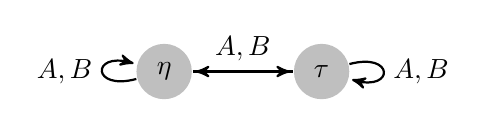
\begin{tikzpicture}[->,>=stealth',shorten >=1pt,auto,node distance=2cm,
      thick]

    \node[vertex] (1) {$\eta$};
    \node[vertex] (2) [right of=1] {$\tau$};
    \path[edge]
          (1) edge node {$A,B$} (2)
              edge [loop left] node {$A,B$} (1)
          (2) edge node {} (1)
              edge [loop right] node {$A,B$} (2);
\end{tikzpicture}
\caption{Our model before $B$ temporarily left the game.}
\label{ambeforefigure}
\end{subfigure}
~
\begin{subfigure}[b]{.45\textwidth}
\centering
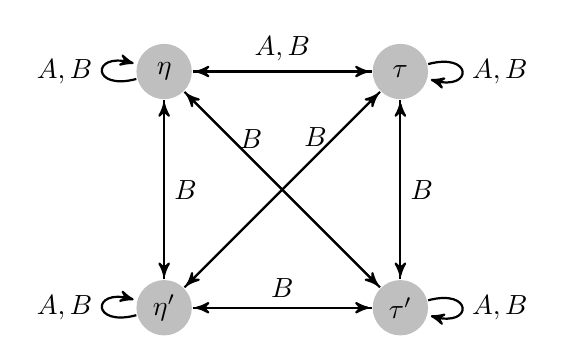
\begin{tikzpicture}[->,>=stealth',shorten >=1pt,auto,node distance=3cm,
      thick]

    \node[vertex] (1) {$\eta$};
    \node[vertex] (2) [right of=1] {$\tau$};
    \node[vertex] (3) [below of=1] {$\eta'$};
    \node[vertex] (4) [right of=3] {$\tau'$};
    \path[edge]
          (1) edge node {$A,B$} (2)
              edge [loop left] node {$A,B$} (1)
							edge node {$B$} (3)
							edge node {} (4)
          (2) edge node {} (1)
              edge [loop right] node {$A,B$} (2)
							edge node [above,pos = 0.33] {$B$} (3)
							edge node {$B$} (4)
					(3) edge node {} (1)
							edge node {} (2)
							edge node {$B$} (4)
							edge [loop left] node {$A,B$} (3)
					(4) edge node [above, pos = 0.66] {$B$} (1)
							edge node {} (2)
							edge node {} (3)
							edge [loop right] node {$A,B$} (4);
\end{tikzpicture}
\caption{Our model after $B$ returns and is unsure about whether $A$ has looked
	at the coin.
$\tau$ and $\eta$ are worlds where $A$ has not cheated while $\tau'$ and $\eta'$
are worlds where $A$ has cheated and looked at the coin.}
\label{amafterfigure}
\end{subfigure}
\caption[Kripke model changes after an informative update]{The differences before and after $B$'s temporary departure.}
\label{amkripkefigure}
\end{figure}

In Figure \ref{amkripkefigure}, we can say that $H$ is true at $\{\eta,\eta'\}$ and $T$ is
true at $\{\tau,\tau'\}$, but that in $\eta'$ and $\tau'$ $A$ has taken a look
at the coin and can distinguish between $\eta'$ and $\tau'$.
Our change in epistemic state is a change that we cannot model with public
announcement logic.
It is a private announcement such that $B$ is aware of the announcement, but not
of its contents.\\
\\
This update is one we can capture with an action model.
$B$ considers it possible that an action where $A$ looks at the coin and learns
$H$ occurs.
He also considers the action where $A$ looks at the coin and learns $T$ possible
as well.
Lastly, he considers that $A$ did not look at the coin and thus the state of the
world remains the same, signified by {\bf tr}.
As $B$ cannot tell which one of them occurred, but is aware that one of them did
occur, he considers them indistinguishable.
We can represent them as a ``possible actions" model, as we show in Figure
\ref{amprivatea}.
Baltag, Moss and Solecki define an operation to execute the model in Figure
\ref{amprivatea} on Figure \ref{ambeforefigure}, yielding Figure
\ref{amafterfigure} \cite{baltag1998lpa}.

\begin{figure}[H]
\centering
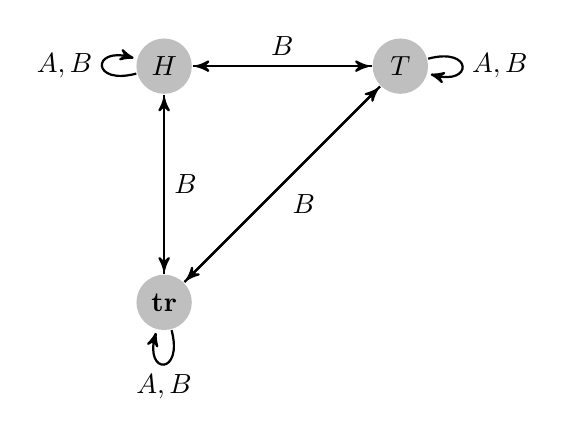
\begin{tikzpicture}[->,>=stealth',shorten >=1pt,auto,node distance=3cm,
      thick]

    \node[vertex] (1) {$H$};
    \node[vertex] (2) [right of=1] {$T$};
    \node[vertex] (3) [below of=1] {{\bf tr}};
    \path[edge]
          (1) edge node {$B$} (2)
							edge node {$B$} (3)
              edge [loop left] node {$A,B$} (1)
          (2) edge node {} (1)
							edge node {$B$} (3)
              edge [loop right] node {$A,B$} (2)
					(3) edge [loop below] node {$A,B$} (3)
							edge node {} (1)
							edge node {} (2);
\end{tikzpicture}
\caption[Example action model]{An example of an action model; in this example, the update models $B$
becoming suspicious of $A$ having learnt whether $H$ or $T$ is true, but not
knowing whether the $A$ actually has not learnt anything and the world remains
as it was before (signified {\bf tr}).}
\label{amprivatea}
\end{figure}

Baltag and Moss extend the action models they proposed with Solecki into classes
of action models, which they term action signatures \cite{baltag2005programs}.
They formalise general descriptions of actions, such as announcements, private
announcements, lying, suspicion and other epistemic updates.
As an example, they generalise all public announcements to a single structure,
showing the superior expressiveness of action models.
They also specify a syntax for discussing actions of a given action signature,
allowing them to generate the logic of public announcements in its entirety.
Within this syntax, the action model structures are used as syntactical objects.
Like van Ditmarsch's epistemic actions, Baltag and Moss' syntax extends previous
logics of dynamics and change.\\
\\
Action models are define a method of execution upon an epistemic model that is well-understood.
The execution will update a model of knowledge from a pre-update to a
post-update state.
Unfortunately, the cost of action model execution (that is, to transform a state
of information to a new state using an update specified by an action model) is
quite high.
It involves taking a Cartesian product of all possible actions.
This indicates that, given $N$ possible actions in an action model, $N^2$
actions must be computed in the new state of information before the model can
be refined.

\subsection{Comparison to relational epistemic actions} \label{epi_compare}
Both relational epistemic actions \cite{hoek2008dynamic} and action models
\cite{baltag1998lpa} describe a larger range of epistemic updates for our game of heads and tails.
The examples we chose earlier, regarding $C$ telling $A$ about the state of the
coin, or $B$ becoming suspicious of $A$ can be expressed using either framework.
What, then, is the real difference between employing action models, as opposed
to relational epistemic actions?\\
\\
van Ditmarsch, van der Hoek and Kooi \cite{hoek2008dynamic}, as well as Baltag and Moss
\cite{baltag2005programs} independently
note that the ``possible actions" of action models  are actually relational
epistemic actions.
In their own review of action models, van Ditmarsch, van der Hoek and Kooi
motivate this with an example.\\
\\
They consider the non-deterministic choice of 3 possible actions which are
indistinguishable externally.
As an example, $B$ might learn that $A$ knows either of $H$ or $T$, or has
learnt nothing at all.
Since $B$ does not know which of these actions could occur, each of these
epistemic updates is a possible action.\\
\\
They show that it is possible to express this uncertainty in a manner quite similar
to an action model.
Similarly, the corresponding action model of whether $B$ learns of $A$'s
knowledge of $H$, $T$ or nothing new is quite easily interpreted in a manner
akin to relational epistemic actions.
Their general result is that relational actions can be expressed as action
models, and vice versa.
As van Ditmarsch, van der Hoek and Kooi have already shown, it is in reasoning
with these models that the models differ.\\
\\
Notably, relational epistemic actions and action models suffer from the same
weakness, in that they are only externally describe an update of information.
Their execution and specification are only useful to a third-party viewer, and
how agents internal to a system update their knowledge is not clear.
This is one of several weaknesses in current dynamic epistemic logic, with
regards to translating a specification of an informational update into an
implementable series of messages.\\
\\
It is in their reasoning that action models and relational epistemic actions
differ most.
action models give us a notion of uncertainty between actions in a manner
similar to the possible worlds model, allowing us to use a formally established framework
to reason about dynamic updates.
This allows us to reason about our updates and their effects in a more natural
and well-understood way.\\
\\
Conversely, van Ditmarsch's relational epistemic actions give us a syntax that
is perhaps more natural than the one Baltag and Moss define.
Baltag and Moss are note that it is non-standard to use the modelling structures
inside a syntax \cite{baltag2005programs}.
In the context of interpreting and making sensible updates, however, it is
perhaps less useful to have abstraction at the cost of useful interpretations,
suggesting that action models are a more interesting way to model epistemic
updates.
Indeed, it would appear that at the moment action models are experiencing more
interest compared to relational epistemic actions, as we explore in the next
section.

\section{Extensions of action models}
Action models, when first introduced in \cite{baltag1998lpa}, were a concept that could be used to make
formal reasonings about actions in a similar way to possible worlds semantics.
Progress in this area has added a syntax that uses action models as syntactic
objects, improved the expressiveness of action models and investigated the
synthesis of action models.
Much of the discussion has showed how powerful action models are as a way for a
third party to reason about an informational update, and improved what kind of
informational updates we can capture.\\
\\
Baltag and Moss \cite{baltag2005programs} define a powerful syntax for constructing epistemic programs.
Their syntax is as powerful as van Ditmarsch's in relational epistemic actions,
being able to express sequences of epistemic actions or make a non-deterministic
choice between two established action models.
In our game, we would be able to model sequences of actions, such as $A$ finding
out whether $H$ is true or $T$ is true while $B$ watches, then $B$ finding out
whether $H$ or $T$ is true but without $A$ being aware of $B$ learning this.\\
\\
The only objection to their syntax, as raised earlier, is the curious use of
the semantic structures within a syntax.
It is also notable that the operations of composition and non-deterministic
choice can be as costly as action model execution, generating $N \times M$
possible actions, given two action models of size $N$ and $M$
respectively \cite{baltag2005programs}.\\
\\
van Benthem, van Eijck and Kooi \cite{benthem2006lcc} extend action models for a new language to
handle communication and change.
Their main contribution here is to improve action model languages with notions
of group knowledge and iterations of an action model's execution.
This logic of communication and change uses previous logics of change as a basis
and proceeds to interpret it in an epistemic fashion.\\
\\
van Ditmarsch, French and Pinchinat \cite{van2009simulation,van2010future} construct a future action model logic in
their contribution.
Together, their work shows how one can determine if for a particular possible
world it is possible to update it such that a condition $\phi$ is true after an
update.\\
\\
In a recent contribution, Hales \cite{hales13synthesis} describes an algorithm that can synthesise arbitrary
action models.
Hales builds upon van Ditmarsch and French's work, showing that if an action
model $\alpha$ exists to ensure a condition $\phi$ was true after that models
execution, then there is a method by which an equivalent action model can be generated.
This contribution is especially notable due to it generalising outside of
epistemic logic, to any modal logic system.\\
\\
This shows that we can use action models to ensure a condition is true
in a new epistemic state, if it is at all possible.
As an example, if in our game of coins $A$ and $B$ are unsure whether $H$ or $T$
are true, we would be able to determine if an action model exists such that
after its execution, $\Box_A H \land \Box_B H$ was true at a
specific world.
Employing the work of Hales' would allow us to synthesise this action model.\\
\\
An alternative approach is shown by Aucher in
\cite{doi:10.3166/jancl.21.289-321,doi:10.1080/11663081.2012.736703}, which is related to
to Hales' work.
Aucher discusses the concepts of epistemic planning.
To define epistemic planning, suppose that we have an information state where
some epistemic sentence $\phi$ is true.
We want to construct an information state such that the epistemic sentence
$\phi''$ is true.
Epistemic planning involves finding an update that moves from $\phi$ to
$\phi''$.
It is very similar to Hales' work, but unlike Hales' action models it allows a
finer degree of control about the situation prior to an event.\\
\\
Aucher provides a framework to infer properties about an update that will
realise $\phi''$ from $\phi$.
What is most interesting is that Aucher provides a framework to reason about the
properties of an update that realises $\phi''$ from $\phi$.
His contribution is novel, but parallel to the work of Hales' since it describes properties of event
models that can affect a change, whilst Hales describes the actual change itself and gives
rudimentary analysis of his procedure.\\
\\
The state of the art in action models and this section of dynamic epistemic
logic is thus focused on improving descriptions of information updates, or how
we can use them to achieve a given epistemic state.
These works focus on action model specification and existence, with very little regard given to
realising their construction in an algorithmic sense.

\section{Belief revision}

Suppose that $A$ and $B$ are playing the heads-or-tails game with $C$ again.
$C$ checks the coin and announces ``The coin is heads up".
$A$ and $B$ now believe that the coin $C$ is holding is heads up.
But $C$ rechecks the coin and realises it is actually {\em tails}.
She apologetically announces to $A$ and $B$ that the coin is actually tails.\\
\\
Our current update frameworks cannot deal with the world being inconsistent with
our knowledge.
The moment that the beliefs and knowledge of an agent must be reconciled with
the world, agents cannot update their knowledge appropriately.
They stop being able to continue the state of the world.\\
\\
We will briefly address the field of dynamic epistemic logic that allows us to revise the epistemic state of the
world.
This field is ``belief revision", where what agents believe to be true can be
revised to match the new state of the world.
Belief revision was first properly introduced by Alchourr{\'o}n in \cite{theLogicOfTheoryChange} and also
expanded on by G{\"a}rdenfors \cite{gairdenfors1988knowledge}.
They discussed the AGM approach, named after Alchourr{\'o}n, G{\"a}rdenfors and Makinson.
AGM captures three concepts --- the ability to {\em expand} the beliefs of agents, to {\em contract}
or reject some subset of their beliefs, or to {\em revise} their beliefs using the smallest, minimal
change to their set of beliefs.
These papers built upon initial frameworks, such as the one Harper discusses in
\cite{harper1976rational}, or the truth maintenance systems for database
consistency which Doyle introduces in \cite{Doyle1979231}.\\
\\
Belief revision is more robust than the frameworks we considered as it allows
for beliefs that are inconsistent with the actual state of the world.
This robustness invites more obvious applications for revision belief in fields such as
artificial intelligence or database management and consistency.
It is a powerful approach in resolving conflicts between knowledge and facts.
This approach is tangential to what we are interested in, however, as we are
examining methods of constructing updates, as opposed to reconciling what we
know and what we have observed.

\section{Refinement quantified modal logics} \label{section:refineModalLogics}

A final, seemingly tangential approach to dynamic epistemic logic is to consider the concept of refinements.
Refinements are a relation between two epistemic Kripke models where the amount of knowledge about
the facts captured in a situation are constant.
Instead, refinements vary the negative knowledge --- the things that agents are uncertain about ---
between the two epistemic situations.
They are a way of describing a partial ordering of the uncertainty in a set of epistemic models.\\
\\
Refinements can be construed as another way of viewing updates; van Ditmarsch and French \cite{van2009simulation} show
that refinements and informative updates are equivalent.
What is most interesting about refinements is the ability to quantify over them.
This means that we can actually quantify over the set of informative updates, and to thus make
reasonings about all updates, or possible updates.\\
\\
van Ditmarsch and French also propose methods to augment existing logics with their quantification
in \cite{van2009simulation}.
van Ditmarsch, French and Pinchinat \cite{van2010future} also combine their work to construct a modal logic augmented
with this quantification, the future event logic.
These steps were the beginning to being able to quantify across informative updates and models.
The intuition behind these results is that queries such as ``does an informative update exist?" or
``all informative updates will fulfill some condition" are decidable.
However, Bozzelli et. al \cite{refineModalComplexity} show that the lower bound on executing such a query is exponential. \\
\\
Hales unifies the work proposed in \cite{van2009simulation}, by proposing an arbitrary action model
logic in \cite{hales13synthesis}.
Hales also completes the semantics for this new logic, by showing that quantification over
refinements is the same as quantifying over updates.\\
\\
These ideas are not directly related to update construction, but later they play a part in forming
models effectively.
We will employ the power of refinement quantification and the semantics given by Hales to
effectively construct action models \cite{hales13synthesis}.

\section{Open questions} \label{section:literatureReview:openQuestions}

We have explored informative updates and different ways of specifying changes, as represented by action models, and examined the state of the
art in informative updates.
Much work has been done on specifying action models and proving their existence and properties.
However, very little work has been done on the construction of action models.
This has limited their usefulness in automated multi-agent systems, and there is little research
with regards to constructing provably correct updates.\\
\\
The question of ``can we construct provably correct updates?" has thus been well-studied.
However, there is still the open question of ``how do we construct provably correct updates?"
The results of this paper are a step towards an answer in this area.

\section{Technical preliminaries}
In order to discuss event model synthesis, we first define essential concepts regarding event
models and the semantics of the logics we are working within.

\subsection{Models}

\begin{defn} \label{frame}
	Let $\Sigma$ be a set of atoms and $R: A \to \mathcal{P}(S \times S)$, a function from agents to
	accessibility relations.
	Then the tuple $(\Sigma, R)$ is a frame.
\end{defn}

A frame represents a mathematical structure, but holds no meaningful information.
In order to give meaning and be able to draw conclusions from the frame, we can
construct a valuation function that transforms the frame into a model detailing
information.
\begin{defn} \label{model}
	Let $L$ be a logical language.
	Let $F = (\Sigma, R)$ be a frame, and $A$ a set of agents.
	In the context of epistemic modal logic, $\Sigma$ is a set of atomic knowledge points.
	Let $V: L \to \mathcal{P}(\Sigma)$ be a function mapping any
	well-formed	sentence in $L$ to a subset of $\Sigma$.
	We say $V$ is a valuation function on $F$.\\
	\\
	Then $\krMo = (F, V) = (\Sigma, R, V)$ is a Kripke
	model.
\end{defn}
A multi-pointed model is a model $\krMo = (\Sigma, R, V)$ with a set of designated states, $T$.
When $T = \{s\}$ is a single state, we say that the model is a pointed model and write $M_s$.
We say $\kripkeClass$ is the class of all Kripke models.

\begin{defn} \label{evModel}
	Let $L$ be a logical language.
	Let $F = (\Sigma, R)$ be a frame, and $A$ a set of agents.
	An event model $\aMod{\evMo = (\Sigma, R, pre)}$ with preconditions defined on $\mathcal{L}$ consists of
	\begin{itemize}
		\item a domain $\aMod{\Sigma}$ of possible atomic action points
		\item an accessibility function, $\aMod{R: A \to \mathcal{P}(\Sigma \times
        \Sigma)}$, a function from agents to
		accessibility relations on $\Sigma$.\\
		We refer to $\aMod{R(a)}$ as $\aMod{R_a}$.
		We will refer to all accessible action points from $\aMod{s}$ as
    $\aMod{s R_a}$, and all action points that
		can access $\aMod{t}$ as $\aMod{R_a t}$.
		Furthermore, we say $\aMod{s R_a t}$ means $\aMod{t}$ is
    $\aMod{a}$-accessible from $\aMod{s}$.
		\item a precondition function, $\aMod{pre: \Sigma} \to \mathcal{L}$ which maps an action point to a
		sentence in $\mathcal{L}$
	\end{itemize}
\end{defn}

We adopt the convention that an event model is written using sans-serif fonts.
Pointed and multi-pointed event models are similarly defined to pointed and multi-pointed Kripke
models.
We adopt the convention for pointed event models that $\aMod{\evMo^1 = (\Sigma^1, R^1,
pre^1, T^1)}$ and $\aMod{\evMo^\alpha =
  (\Sigma^\alpha,R^\alpha,pre^\alpha,T^\alpha)}$.
Furthermore, in literature both of the terms event models and action models are used to describe
the same concept, and we use them interchangeably throughout this paper to refer to event models.

\begin{defn} \label{evModelEx}
Let $\kripkeClass = (\Sigma, R, V) \in \kripkeClass$. We define event model
execution for an event model $\aMod{\evMo = (\Sigma,
		R, pre)} \in
\eventClass$ as follows.
The result of executing $\evMo$ on the model $\krMo$ is denoted by $M \otimes N = M' = (\Sigma', R', V')$ where
\begin{itemize}
	\item $\Sigma' = \{(s,\aMod{u}) | s \in \Sigma, \aMod{u \in
    \Sigma} \text{ such that } M_s \models \aMod{pre(u)}\}$
	\item $(s, u) R_a' (t, v) \iff s R_a t \land \aMod{u R_a v}$
	\item $V'((s,u)) = V(s)$
\end{itemize}
We define pointed event model execution as $\krMo_s \otimes
\aMod{\evMo_u}
= (\krMo \otimes \aMod{\evMo})_{(s, \aMod{u})}$.
This pointed model execution is only sensible if and only if $M_s \models
\aMod{pre(u)}$ and thus $(s,\aMod{u})
	\in \Sigma'$.
\end{defn}

We say $\eventClass$ is the class of all event models.

\begin{defn} \label{pub}
Let $\aMod{\evMo = (\{ \sigma \}, R, \{ (\sigma, \phi)\}})$ be an event model.
Let $\aMod{\sigma}$ be a single action point and $\aMod{R_a =
  \{(\sigma, \sigma)\}}$ for each $a \in A$ and $\phi
\in \mathcal{L}$.
Then $M$ is a public announcement of $\phi$.
We say $\publicAnnClass$ is the class of all action models that
are public announcements of a sentence in $L$.
\end{defn}

\begin{defn} \label{insanity}
Let $\aMod{\evMo = (\{ \sigma \}, \varnothing, \{(\sigma, \phi)\})}$ be an action model
where $\phi \in L$ and $\aMod{\sigma}$ is an action point.
$\aMod{\evMo}$ represents the truthful announcement of $\phi$ causing all agents to renounce all their beliefs.
$\insaneClass = \{\aMod{\evMo} | \phi \in L\}$ is the class of all such action models.
\end{defn}
We call this class of models ``insanity models".
This is because after the execution of an insanity model, all agents have renounced every belief
they hold.
They thus believe in everything --- that both propositions $p$ and $\neg p$ hold.
Allowing them to believe such contradictions means that they are effectively insane.

\subsection{Bisimilarity, simulation and refinement}

\begin{defn} \label{bisimKripke}
	Let $\krMo$, $\krMo'$ be Kripke models and $\sim \subseteq \Sigma \times \Sigma'$ be a non-empty binary
	relation such that
	\begin{itemize}
		\item {\bf atoms}: for each $s \in \Sigma$ and $s' \in \Sigma'$ such that $s \sim s'$, $V(s) = V'(s')$
		\item {\bf front-$a$}: for each $s \in \Sigma$ such that $s \sim s'$, for each $t$ such that
		$s R_a t$ then there exists $t'$ such that $s' R_a' t'$ and $t \sim t'$
		\item {\bf back-$a$}: for each $s' \in \Sigma'$ such that $s \sim s'$, for each $t$ such that
		$s' R_a' r'$ then there exists $t$ such that $s R_a t$ and $t \sim t'$
	\end{itemize}
	$\sim$ is a bisimulation between $M$ and $M'$ if and only if {\bf atoms} holds and {\bf front-$a$}
	and {\bf back-$a$} hold for each $a \in A$.
	We denote $M$ and $M'$ being bisimilar by $M \sim M'$.
\end{defn}
% \FIXME: add in citations

\begin{lemma} \label{bisimEquivalence}
	The relation $\sim$ is an equivalence relation.
\end{lemma}

This is a well-known result.
See \cite{blackburn2002modal} by de Rijke, Venema and Blackburn for further reading..

\begin{defn} \label{nBisimKripke}
Let $\krMo_s, \krMo'_{s'} \in \kripkeClass$.
We define $n$-bisimilarity inductively as follows.
We say that $\krMo_s$ is $0$-bisimilar to $\krMo'_{s'}$ if and only if $V(s) = V'(s)$.
Then for $n > 0$ we say that $\krMo_s$ is $n$-bisimilar to $\krMo'_{s'}$ if and only if for every $a \in A$
\begin{itemize}
	\item $M_s$ is $n-1$-bisimilar to $M'_{s'}$
	\item {\bf $n$-front-$a$}: for each $t \in s R_a$, there is a $t' \in s' R'_a$ such that $M_t$ is
	$n-1$-bisimilar to $M'_{t'}$
	\item {\bf $n$-back-$a$}: for each $t' \in s' R'_a$ there is a $t \in s R_a$ such that $M_t$ is
	$n-1$-bisimilar to $M'_{t'}$
\end{itemize}
We denote $\krMo_s$ and $\krMo'_{s'}$ being $n$-bisimilar by $\krMo_s \sim_n
\krMo'_{s'}$.
\end{defn}
For a multi-pointed Kripke model $\krMo_T$ and $\krMo'_{T'}$, we have that
$\krMo_T \sim_n
\krMo'_{T'}$ if and only if for each point $t \in T$ there is a point $t' \in T'$
such that $\krMo_t \sim_n \krMo'_{t'}$ and vice versa.

\begin{defn} \label{refinement}
Let $B \subseteq A$ and $\krMo$ and $\krMo'$ be Kripke models. A non-empty relation $\lesssim \subseteq \Sigma
\times \Sigma'$ is a $B$-simulation if and only if it satisfies {\bf atoms}, {\bf forth-$a$} for
every $a \in A$ and {\bf back-$a$} for every $a \in A \setminus B$.
\end{defn}
If $(\sigma, \sigma') \in \lesssim$ then we say $\krMo'_{\sigma'}$ is a
$B$-simulation of $\krMo_\sigma$ and
$\krMo_\sigma$ a $B$-refinement of $\krMo'_{\sigma'}$.
We write $\krMo_{\sigma} \lesssim \krMo'_{\sigma'}$ or equivalently
$\krMo'_{\sigma'} \gtrsim \krMo_{\sigma}$.

\begin{lemma} \label{refinementPreorder}
The relation $\lesssim_B$ is a preorder.
\end{lemma}
This is shown by van Ditsmarch and French in \cite{van2009simulation}.

\begin{lemma} \label{bisimilarIsRefinement}
Let $\krMo_\sigma, \krMo'_{\sigma'} \in \kripkeClass$ and $B \subseteq A$.
Then $\krMo_\sigma \sim \krMo'_{\sigma'} \implies \krMo_\sigma \lesssim_B \krMo'_{\sigma'}$.
\end{lemma}

This follows trivially from Definition \ref{refinement} and Definition \ref{bisimKripke}.

\begin{defn} \label{brestrict}
Let $B \subseteq A$ and let $\aMod{\evMo} \in \eventClass$. Then $\aMod{\evMo}$ is a $B$-restricted event model if and
only if for every $\aMod{u \in \Sigma}$ and every $\krMo_s \in \kripkeClass$
such that $\krMo_s \models pre(u)$ we
have $\krMo_s \otimes \evMo_u \gtrsim_B \krMo_s$.
We say the class of $B$-restricted action models is $\eventClass_B$.
\end{defn}

\FIXME: citation here

\subsection{Language semantics}
We now discuss the semantics and syntax of several different languages, culminating with language of
arbitrary action model logic which will rely upon each of the languages we discuss.

\begin{defn} \label{propLogic}
Let $\krMo = (\Sigma, R, V) \in \kripkeClass$.
The language of propositional logic $\langProp$ is inductively defined by
\[
	\phi ::= p \text{ } | \text{ } \neg \phi \text{ } | \text{ } (\phi \land \phi)
\]

The interpretation of $\phi \in \langProp$ in the logic $K$ is defined inductively as

\begin{itemize}
	\item $\krMo_s \models p$ iff $p \in V(s)$
	\item $\krMo_s \models \neg \phi$ iff $\krMo_s \not \models \phi$
	\item $\krMo_s \models \phi \land \psi$ iff $\krMo_s \models \phi$ and $\krMo_s \models \psi$
\end{itemize}

for $s \in \Sigma$.
\end{defn}

We will adopt the standard abbreviations for propositional logic, such as $\phi \lor \phi =
\neg(\neg \phi \land \neg \phi)$.
These are defined in \cite{blackburn2002modal}.

\begin{defn} \label{modalLogic}
Let $\krMoM = (\Sigma, R, V) \in \kripkeClass$.
The language of modal logic $\lang$ is $\langProp$ with the additional inductive case
\[
	 \Box_a \phi
\]
The interpretation of $\phi \in \lang$ in the logic $K$ is the same as $\langProp$, with the
additional inductive case
\[
	\krMo_s \models \Box_a \phi \text{ iff for every }t \in s R_a: \krMo_t \models \phi
\]
for $a \in A$ and $s \in \Sigma$.
\end{defn}
The Kripke semantics for modal logic are well-known.
We will adopt the standard abbreviations for Kripke semantics --- see \cite{blackburn2002modal}.\\
\\
In epistemic logics, the formula $\Box_a \phi$ is often read as ``$a$ knows/believes $\phi$", while
its dual operator, $\Diamond_a \phi$ means ``$a$ considers $\phi$ possible".
We also employ the abbreviation $\Box_B \phi$ where $B \subseteq A$ to be $\bigwedge_{b \in B}
\Box_b \phi$.
In the case where $B = A$ we write $\krMo_s \models \Box \phi$.\\
\\
We say that a formula $\phi$ is satisfied by a pointed model Kripke model $\krMo_s \in \kripkeClass$ iff
$\krMo_s \models \phi$.
We say that $\phi$ is satisfied by a model $\krMo = (\Sigma, R, V)$ (denoted by
    $\krMo \models \phi$) iff
for all $\sigma \in \Sigma$, $\krMo_\sigma \models \phi$.
Furthermore, $\phi$ is valid in a class of Kripke models $\kripkeClass$ iff for
every model $\krMo \in
\kripkeClass$, $\krMo \models \phi$.\\
\\
%\FIXME: Add citation
In addition to $\Box_a$ we introduce the cover operator $\cover_a$, following the definition used in
\cite{venemaproofsystems}.
\begin{defn} \label{coverDef}
Let $\Gamma \subseteq \lang$ be a finite set of formulae.
Then
\[
  \cover_a \Gamma \hat{=} \Box_a \bigvee_{\gamma \in \Gamma} \gamma \land
  \bigwedge_{\gamma \in \Gamma} \Diamond_a \gamma
\]
Similarly, if $B \subseteq A$, then $\cover_B \Gamma \hat{=} \bigwedge_{b \in B}
\cover_b \Gamma$.
\end{defn}
We note that this is a simple abbreviation, and we can define $\Box_a$ and
$\Diamond_a$ in terms of it.
$\Box_a \phi \iff \cover_a \phi \lor \cover_a \varnothing$, while $\Diamond_a
\phi \iff \cover_a \{\phi, \top\}$.
$\cover$ is the basis for the axiomatisation of refinement modal logic.\\
\\
Finally, we discuss modal depth.
We define modal depth as follows
\begin{defn} \label{modalDepth}
We define the modal depth of a formula $\phi \in \lang$ ($MD(\phi)$) as follows
\begin{itemize}
	\item $\mDep(p) = 0$ for atomic formula $p$
	\item $\mDep(\top) = \mDep(\bot)$
	\item $\mDep(\neg \phi) = \mDep(\phi)$
	\item $\mDep(\phi \land \psi) = MAX(\mDep(\phi), \mDep(\psi))$
	\item $\mDep(\Box_a \phi) = 1 + \mDep(\phi)$
\end{itemize}
\end{defn}

Next, we build upon our logics to introduce the concepts updates and refinements as modal logics.
We begin by introducing action model logic, as first defined by Baltag, Moss and Solecki in
\cite{baltag1998lpa}.

\begin{defn} \label{actModelLogic}
Let $\krMo = (\Sigma, R, V) \in \kripkeClass$ be a Kripke model and $\aMod{\evMo
  = (\Sigma, R, pre)} \in
\eventClass$ a multi-pointed event model.
The interpretation of $\phi \in \langActEx$ is the same as its interpretation in $\lang$
(\ref{modalLogic}), but with the additional
inductive cases
\begin{itemize}
	\item $\krMo_s \models \sqex{\aMod{\evMo_\sigma}} \phi$ iff $\krMo_s \models
  \phi \implies \krMo_s \otimes \aMod{\evMo_\sigma} \models
	\phi$ (see Definition \ref{evModelEx})
	\item $\krMo_s \models \sqex{\aMod{\evMo_T}} \phi$ iff for every $\aMod{\sigma
    \in T}$, $\krMo_s \models \sqex{\aMod{\evMo_\sigma}} \phi$ 
\end{itemize}
\end{defn}
$\sqex{\aMod{\evMo_\sigma}} \phi$ can be read as ``the successful execution of the informative update modelled by
$\aMod{\evMo_\sigma}$ will result in $\phi$ being true".
Similarly, $\sqex{\aMod{\evMo_T}} \phi$ can be read as ``the successful execution of the informative update
modelled by $\aMod{\evMo_T}$ will result in $\phi$ being true".
If $\aMod{T = \Sigma}$ then we write $M_s \models \sqex{\aMod{\evMo}} \phi$.\\
\\
We adopt the standard convention for the dual operators, with $\anex{
  \aMod{\evMo_\sigma} } \phi$ being
read as ``the successful execution of the informative update modelled by
$\aMod{\evMo_\sigma}$ may result in
$\phi$ being true".
Again, $\anex{ \aMod{\evMo_T} } \phi$ can be read as ``the successful execution of the informative
update modelled by $\aMod{\evMo_T}$ may result in $\phi$ being true".\\
\\
We also introduce refinement modal logic, as first introduced by van Ditmarsch and French in
\cite{van2009simulation}.

\begin{defn} \label{refineLogic}
Let $\krMo = (\Sigma, R, V) \in \kripkeClass$ be a Kripke model.
The interpretation of $\phi \in \langRefine$ in the logic $K_\forall$ is the same as $\lang$
(\ref{modalLogic}), but with the additional inductive case
\[
	\krMo_s \models \forall_B \phi \text{ iff } \forall \krMo'_{s'} \in
  \eventClass \text{ such that } \krMo'_{s'}
	\lesssim_B \krMo_s : \krMo'_{s'} \models \phi
\]
\end{defn}
We read the formula $\forall_B \phi$ as ``for any $B$-refinement, $\phi$ will hold".
Its dual, $\exists_B \phi$ can be read as ``there is a $B$-refinement such that $\phi$ will hold".
As in the previous operations, when $B = A$ we will write $\forall \phi$.
In addition, when $B = \{b\}$ we write $\forall_b$ and $\exists_b$.
Our text interpretation is taken from an interpretation used by Hales, French and Davies in \cite{hales2012refinement}.

\begin{defn} \label{arbActLogic}
The language of arbitrary action model logic, $\langArbAct$ is first defined in \cite{hales13synthesis}.
We inductively define $\langArbAct$ by
\[
	\phi ::= p \text{ } | \text{ } \neg \phi \text{ } | \text{ } \phi \land \phi \text{ } | \text{ } \Box_a \phi \text{ } |
  \text{ }\sqex{N_T} \phi \text{ } | \text{ } \forall_B \phi
\]
for $\aMod{\evMo_T} \in \eventClass$ and $B \subseteq A$.
\end{defn}
$\langArbAct$ is $\langActEx$ with $\forall_B$ and is also $\langRefine$ with $\sqex{N_T}$.

%\FIXME: Add in James' alternate definition for \forall

% \FIXME: Need more motivating text.
\subsubsection{Miscellaneous Semantic Results}
We provide other results that we will use in the main technical findings of this paper.

\begin{defn} \label{bisimEvent}
	Let $\aMod{\evMo, \evMo'} \in \eventClass$ with preconditions defined on $\langArbAct$.
	A non-empty relation $\sim$ on $\aMod{\evMo} \times \aMod{\evMo'}$ is a bisimulation if and only if for every $a \in A$
	and $\aMod{(s, s') \in \sim}$, the following three conditions hold:
	\begin{itemize}
		\item {\bf pre}: $\aMod{pre(s)} \iff \aMod{pre'(s')}$
		\item {\bf forth-$a$}: for every $\aMod{v \in s R_a}$ there is a $\aMod{v'
      \in s' R'_a}$ such that $\aMod{(v,v')} \in \sim$
		\item {\bf back-$a$}: for every $\aMod{v' \in s' R'_a}$ there is a $\aMod{v
      \in s R_a}$ such that $\aMod{(v,v')} \in
		\sim$
	\end{itemize}
	If $\aMod{(s, s') \in \sim}$ we write $\aMod{\evMo_s \sim '\evMo_{s'}}$ to
  denote that $\evMo_s$ and $\evMo'_{s'}$ are bisimilar and
	that there is a bisimulation between $\evMo_s$ and $\evMo'_{s'}$.
\end{defn}

\begin{lemma} \label{eventModelsRefine}
Let $M_\sigma \in \eventClass$ be an event model and let $N_s \in \kripkeClass$ be a Kripke
model such that $N_s \models pre(\sigma)$.
Then $N_s \otimes M_\sigma \lesssim N_s$.
\end{lemma}

\begin{lemma} \label{eventModelEquivalent}
Let $M_\sigma$, $M'_{\sigma'} \in \eventClass$ be event models such that $M_\sigma \sim M'_{\sigma'}$
and let $N_s \in \kripkeClass$ such that $N_s \models pre(\sigma)$.
Then $N_s \otimes M_\sigma \sim N_s \otimes M'_{\sigma'}$.
\end{lemma}

\begin{lemma} \label{nBisimilarKripkeExec}
Let $M_s$, $M'_{s'} \in \kripkeClass$ and $\phi \in \lang$ such that the modal depth of $\phi$,
$MD(\phi) \leq n$.
Suppose that $M_s \sim_{2n} M'_{s'}$ and let $N_t \in
\eventClass$ such that $pre^N(t)$ is of modal depth $n$.
Then $M_s \otimes N_t \models \phi \iff M'_{s'} \otimes N_t \models \phi$.
\end{lemma}

\begin{proof}
We use an inductive proof on the complexity of $\phi$.
We inductively show that $M^1_{(s,t}) = M_s \otimes N_t \models \phi \iff M^2_{(s',t)} = M'_{s'}
\otimes N_t \models \phi$.\\
\\
For our base case, suppose $\phi = p$, where $p$ is an atomic proposition and let
$M^1_{(s,t)} \models \phi$.
\begin{align}
  & \iff p \in V^1_((s,t)) \label{baseOne} \\
  & \iff p \in V(s) \label{baseTwo} \\
  & \iff p \in V'(s) \label{baseThree} \\
  & \iff p \in V^2((s',t)) \label{baseFour} \\
  & \iff M^2_{(s',t)} \models \phi \label{baseFive}
\end{align}
(\ref{baseOne}) follows from the definition of a Kripke model (Definition
\ref{model}).
(\ref{baseTwo}) follows from the definition of event model execution
(Definition \ref{evModelEx}).
(\ref{baseThree}) follows from hypothesis, as $M_s \sim_{2n} M'_{s'} \implies M_s \sim_0 M'_{s'}$
(Definition \ref{nBisimKripke}).
(\ref{baseFour}) follows from the definition of event model execution and
(\ref{baseFive}) follows from the definition of Kripke model (Definition
\ref{model}).
Therefore, we have $M^1_{(s,t)} \models \phi \implies M^2_{(s',t)}$.
The converse follows a similar argument.\\
\\
We handle each of the inductive cases separately now.
Let $\phi = \neg \psi$.
Suppose $M^1_{(s,t)} \models \phi$.
\begin{align}
	& \implies \neg (M^1_{(s,t)} \models \psi) \label{nBisKriNeg1} \\
	& \implies \neg (M^2_{(s',t)} \models \psi) \label{nBisKriNeg2}
\end{align}
(\ref{nBisKriNeg1}) follows from the semantics of propositional logic and the inductive case for
$\neg$ (Lemma \ref{propLogic}).
(\ref{nBisKriNeg2}) follows from the induction hypothesis.\\
\\
Let $\phi = \psi_1 \land \psi_2$.
Suppose $M^1_{(s,t)} \models \phi$.
\begin{align}
	& \implies M^1_{(s,t)} \models \psi_1 \label{nBisKriConj1} \\
	& \iff M^2_{(s',t)} \models \psi_1 \label{nBisKriConj2}
\end{align}
(\ref{nBisKriConj1}) follows from the semantics of propositional logic and the inductive case for
$\land$ (Lemma \ref{propLogic}).
(\ref{nBisKriConj2}) follows from the induction hypothesis.\\
\\
We can employ a similar argument to show that $M^2_{(s',t)} \models \psi_2$ and together with
(\ref{nBisKriConj2}) we have $M^2_{(s',t)} \models \psi_1 \land M^2_{(s',t)} \models \psi_2 \implies
M^2_{(s',t)} \models \psi_1 \land \psi_2 = \phi$.\\
\\
Now, let $\phi = \Diamond_a \psi$ and suppose $M^1_{(s,t)} \models \phi$.
\begin{align}
	& \implies M^1_{(u,v)} \models \psi \text{ for some $(u,v) \in (s,t) R^1_a$} \label{nBisKriMod1} \\
	& \implies M^1_{(u,v)} \models \psi \text{ for some $u \in s R_a$ and $v \in R^N_a$ and $M_s
		\models pre(t)$ and $M_u \models pre(v)$} \label{nBisKriMod2}
\end{align}
(\ref{nBisKriMod1}) follows from the semantics of modal logic and the inductive case for
$\Diamond_a$ (Lemma \ref{modalLogic}).
(\ref{nBisKriMod2}) follows from the definition of event model execution (Definition
		\ref{evModelEx}).\\
\\
From our hypothesis, given that $pre(t) \leq m$ we have that $M_s \sim_{2n} M'_{s'} \implies (M_s \models pre(t) \iff M'_{s'} \models
pre(t))$.
But by the definition of $n$-bisimilarity (Definition \ref{nBisimKripke}), $M_u$ is
$2n-1$-bisimilar to some point $M'_{u'}$.
If $MD(pre^N(v)) \leq n-1$ we have by our induction hypothesis that $M_u \models pre(v) \iff M'_{u'}
\models pre(v)$.\\
\\
Then by the induction hypothesis, $M_u \sim_{2n} M'_{u'} \land MD(\psi) \leq k \implies
M^2_{(u',v)}  \models \psi$.
By the semantics of modal logic (Lemma \ref{modalLogic}) we have that $M^2_{(s',t)} \models
\Diamond_a \psi \implies M^2_{(s',t)} \models \phi$.
\end{proof}

\begin{defn} \label{nBisimEvent}
	Let $M_s, M'_{s'} \in \eventClass$ with preconditions defined on $\langArbAct$.
	We inductively define $n$-bisimilarity for event models.
	We say $M_s$ is $0$-bisimilar to $M'_{s'}$ if and only if $pre(s) \iff pre'(s')$.
	Then for $n>0$ $M_s$ is $n$-bisimilar to $M'_{s'}$ if and only if each of the following hold
	\begin{itemize}
		\item $M_s$ is $n-1$-bisimilar to $M'_{s'}$
		\item {\bf $n$-forth-$a$} for every $t \in s R_a$, there is a $t' \in s' R'_a$ such that $M_t$ is
		$n-1$-bisimilar to $M'_{t'}$
		\item {\bf $n$-back-$a$} for every $t' \in s' R'_a$, there is a $t \in s R_a$ such that $M_t$ is
		$n-1$-bisimilar to $M'_{t'}$
	\end{itemize}
	We write $M_s \sim_n M'_{s'}$ to denote that $M_s$ is $n$-bisimilar to $M'_{s'}$.
\end{defn}

For a multi-pointed event model $M_T$ and $M'_{T'}$, we have that $M_T \sim_n
M'_{T'}$ if and only if for each point $t \in T$ there is a point $t' \in T'$
such that $M_t \sim_n M'_{t'}$ and vice versa.

\begin{lemma} \label{nBisimilarEventExec}
	Let $M_s, M'_{s'} \in \eventClass$ such that $M_s \sim_n M'_{s'}$ and $N_t \in \kripkeClass$.
	For any $\phi \in \lang$ with modal depth $MD(\phi) \leq n$ then $N_t \otimes M_s \models \phi
	\iff N_t \otimes M'_{s'} \models \phi$.
\end{lemma}

\begin{proof}
We use an inductive proof on the complexity of $\phi$.
We inductively show that $M^1_{(t,s}) = N_t \otimes M_s \models \phi \iff M^2_{(t,s')} = N_t \otimes
M'_{s'} \models \phi$.\\
\\
We begin with a base case of $\phi = p$, a single atomic proposition.
Suppose $M^1_{(t,s)} \models \phi$.
Then
\begin{align}
	& \implies p \in V^1_{(t,s)} \label{nBisEvbase1} \\
	& \implies p \in V(t) \label{nBisEvbase2} \\
	& \implies N_t \models pre(s) \label{nBisEvbase4} \\
	& \implies N_t \models pre'(s') \label{nBisEvbase5} \\
	& \implies p \in V^2_{(t,s')} \label{nBisEvbase6}\\
	& \implies M^2_{(t,s')} \models \phi \label{nBisEvbase7}
\end{align}
(\ref{nBisEvbase1}) follows from the semantics for propositional logic (Definition \ref{propLogic}).
(\ref{nBisEvbase2}) and (\ref{nBisEvbase4}) follows from the definition of event model execution (Definition
\ref{evModelEx}).
(\ref{nBisEvbase5}) follows from hypothesis and the definition of $n$-bisimilarity (Definition
\ref{nBisimEvent}).
(\ref{nBisEvbase6}) follows from the definition of event model execution (Definition
\ref{evModelEx}).
Thus, (\ref{nBisEvbase7}) follows from the semantics of propositional logic (Definition
\ref{propLogic}).\\
\\
We go through each of the inductive cases.
Let $\phi = \neg \psi$, and suppose $M^1_{(t,s)} \models \phi$.
Then
\begin{align}
	& \implies \neg (M^1_{(t,s)} \models \psi) \label{nBisEvNeg1} \\
	& \implies \neg (M^2_{(t,s')} \models \psi) \label{nBisEvNeg2} \\
	& \implies M^2_{(t,s')} \models \neg \psi \label{nBisEvNeg3} \\
	& \implies M^2_{(t,s')} \models \phi \label{nBisEvNeg4}
\end{align}
(\ref{nBisEvNeg1}) follows from the semantics of propositional logic (Lemma \ref{propLogic}).
(\ref{nBisEvNeg2}) follows from the induction hypothesis.
(\ref{nBisEvNeg3}) again follows from the semantics of propositional logic (Definition
		\ref{propLogic}) and (\ref{nBisEvNeg4}) is obvious.\\
\\
Let $\phi = \psi_1 \land \psi_2$ and suppose $M^1_{(t,s)} \models \phi$.
Then
\begin{align}
	& \implies M^1_{(t,s}) \models \psi_1 \label{nBisEvCon1} \\
	& \implies M^2_{(t,s'}) \models \psi_1 \label{nBisEvCon2}
\end{align}
(\ref{nBisEvCon1}) follows from the semantics of propositional logic (Lemma \ref{propLogic}).
(\ref{nBisEvCon2}) follows from the induction hypothesis.
Employing a similar process allows us to show that $M^2_{(t,s'}) \models \psi_2$ and together they 
show that $M^2_{(t,s')} \models \phi$.\\
\\
Our final inductive case is to let $a \in A$ and $\phi = \Diamond_a \psi$.
Suppose that $M^1_{(t,s)} \models \phi$.
\begin{align}
	& \iff M^1_{(t,s)} \models \Diamond_a \psi \label{nBisEvMod1} \\
	& \iff M^1_{(v,u)} \models \psi \text{ for some $(v,u) \in (t,s) R^1_a$} \label{nBisEvMod2} \\
	& \iff M^1_{(v,u)} \models \psi \text{ for $v \in t R^N_a$ and $u \in s R_a$ and $N_t \models
		pre(s)$ and $N_v \models pre(u)$} \label{nBisEvMod3} \\
\end{align}

As $M_s \sim_n M'_{s'}$, then there is some $u' \in s R'_a$ such that $M_u \sim_{n-1} M'_{u'}$.
Then we have that $N_v \models pre(u) \iff N_v \models pre'(u)$, since $M_u \sim_{n-1} M'_{u'}
\implies M_u \sim_0 M'_{u'}$.
Then by our induction hypothesis we have that $M^1_{(v,u)} \models \psi \iff M^2_{(v, u')} \models
\psi$.
From this we have (by the semantics of modal logic, in Definition \ref{modalLogic}) $M^2_{(v,u')}
\models \psi \implies M^2_{(t,s')} \models \Diamond_a \psi$.
\end{proof}

%\FIXME: WHO?! Please cite.

\begin{defn} \label{coverNormal}
A formula in cover disjunctive normal form is defined inductively as

\[
	\alpha ::= \pi \land \bigwedge_{b \in B} \cover_b \Gamma_b \text{ } | \text{ } \alpha \lor \alpha
\]

where $\pi \in \langProp$, $B \subseteq A$ and for every $b \in B$, $\Gamma_b$ is a finite set of
formulae in cover disjunctive normal form.
\end{defn}

We note that the above has a base case when $\alpha = \pi$, that is when $B = \varnothing$ or for
each $b \in B \implies \Gamma_b = \varnothing$.

\begin{lemma} \label{allInCoverNormal}
Every formula of $\lang$ is equivalent to a formula in cover disjunctive normal form.
\end{lemma}

This is shown by Bozelli et. al in \cite{DBLPjournalscorrabs12023538}.

\subsection{Axiomatisations}
We will present axiomatisations derived by Hales for $\langArbAct$.
To construct this axiomatisation, we first begin by presenting an axiomatisation for $\lang$, an
axiomatisation for $\langActEx$ and an axiomatisation for $\langRefine$.\\
\\
We say that a formula $\phi$ is provable under an axiomatisation if and only if it can be derived by
some finite sequence of axioms and rules within that axiomatisation.
We denote that $\phi$ is provable by $\vdash \phi$.
When discussing provability, it should be contextually clear which axiomatisation we are using.

\begin{defn} \label{axiomK}
The axiomatisation \AXK consists of the following axioms
\begin{alignat*}{2}
	& \axP && \quad \text{All propositional tautologies} \\
	& \axK && \quad \Box_a(\phi \implies \psi) \implies (\Box_a \phi \implies \Box_a \psi)
\end{alignat*}
and the following rules
\begin{alignat*}{2}
	& \axMP && \quad \text{From $\vdash \phi \implies \psi$ and $\vdash \phi$, infer $\vdash \psi$} \\
	& \axNecK && \quad \text{From $\vdash \phi$, infer $\vdash \Box_a \phi$}
\end{alignat*}
\end{defn}

\begin{lemma} \label{axiomKSoundComplete}
The axiomatisation \AXK is sound and complete with respect to the logic $\lang$.
\end{lemma}

\begin{defn} \label{axiomAML}
The axiomatisation \AXAML contains the axioms and rules from \AXK, as well as the following axioms
\begin{alignat*}{2}
	& \axAP && \quad \sqex{M_\sigma}\pi \iff (pre(\sigma) \implies \pi) \text{ for $\pi \in \langProp$}\\
	& \axAN && \quad \sqex{M_\sigma} \neg \phi \iff (pre(\sigma) \implies \neg \sqex{M_\sigma} \phi)\\
	& \axAC && \quad \sqex{M_\sigma}(\phi \land \psi) \iff (\sqex{M_\sigma}\phi \land \sqex{M_\sigma}\psi\\
	& \axAK && \quad \sqex{M_\sigma}\Box_a\phi \iff (pre(\sigma) \implies \bigwedge_{v \in \sigma R_a}
		\Box_a \sqex{M_v} \phi) \\
	& \axAU && \quad \sqex{M_T} \phi \iff \bigwedge_{u \in T} \sqex{M_u} \phi
\end{alignat*}
and the rule
\[
	\axNecA \quad \text{From $\vdash \phi$ infer $\vdash \sqex{M_\sigma} \phi$}
\]
\end{defn}

\begin{lemma} \label{axiomAMLSoundComplete}
The axiomatisation \AXAML is sound and complete with respect to the logic $\langActEx$.
\end{lemma}

\begin{defn} \label{axiomRML}
The axiomatisation \AXRML contains the axioms and rules from \AXK, as well as the following axioms
\begin{alignat*}{2}
	& \axR && \quad \forall_B (\phi \implies \psi) \implies (\forall_B \phi \implies \forall_B \psi) \\
	& \axRP && \quad \forall_B \pi \iff \pi \text{ where } \pi \in \langProp \\
	& \axRK && \quad\exists_B \cover_a \Gamma_a \iff \bigwedge_{\gamma \in \Gamma} \Diamond_a \exists_B
	\gamma \text{ where } a \in B \\
	& \axRComm && \quad \exists_B \cover_a \Gamma_a \iff \cover_a \{ \exists_B \gamma | \gamma \in
	\Gamma_a\} \text{ where } a \notin B\\
	& \axRDist && \quad \exists_B \bigwedge_{c \in C} \cover_c \Gamma_c \iff \bigwedge_{c \in C}
	\exists_B \cover_c \Gamma_c \text{ where } C \subseteq A
\end{alignat*}
and the rule
\[
	\axNecR \quad \text{From $\vdash \phi$, infer $\vdash \forall_B \phi$}
\]
\end{defn}

\begin{lemma} \label{axiomRMLSoundComplete}
The axiomatisation \AXRML is sound and complete with respect to the logic $\langRefine$.
\end{lemma}

\begin{defn} \label{axiomAAML}
The axiomatisation \AXAAML contains the axioms and rules from \AXRML and \AXAML.
\end{defn}

\begin{thm} \label{axiomAAMLSoundComplete}
The axiomatisation \AXAAML is sound and complete with respect to the logic $\langArbAct$.
\end{thm}

\section{Multi-agent epistemic goal achievement in $\langArbAct$}

In this chapter, we examine an algebra for constructing event models that will, if possible, achieve
epistemic goals or cause a model to crash in the process.
We examine this goal achievement for a subset of agents $B \subseteq A$.\\
\\
%\FIXME: citations here
In \cite{hales13synthesis}, Hales demonstrates that it is possible to determine whether an
finite epistemic goal can be achieved.
Furthermore, if it is achievable Hales constructs event models that will realise
that goal.
We will focus on defining a framework that constructs these event models in a
recursive manner.
This facilitates an automated method for updating knowledge models to reflect a
knowledge state.

\subsection{Technical preliminaries}

The event models that Hales employs resemble finite trees.
We give a rigourous definition for them as follows

\begin{defn} \label{finTree}
Let $M = (\Sigma, R, pre, r)$ be a pointed event model.
$M$ is a finite tree event model if
\begin{itemize}
	\item $\Sigma$, the set of action points is finite
	\item $r$ is the root of the tree and is not accessible from any other action point
	\item for each $s \in \Sigma \setminus \{ r \}$ there is a unique agent $a \in A$ and a unique
	action $p \in \Sigma$ such that $(p,s) \in R(a)$
	\item for each $s \in \Sigma$ there exists a unique sequence of actions in $\Sigma$, $r = s_0,
	s_1, \ldots, s_n = s$ and a sequence of agents $a_1, a_2, \ldots, a_n$ such that $s_0 R_{a_1}
	s_1$, $s_1 R_{a_2} s_2$, $\ldots, s_{n-1} R_{a_n} s_n$
\end{itemize}
\end{defn}

\begin{lemma} \label{insaneIsTree}
The event model class $\insaneClass$ is contained within the event model class
$\treeClass$, that is $\insaneClass \subseteq \treeClass$.
\end{lemma}

It is clear that by our earlier definitions, an insanity event model is also a finite forest event
model.

We say that the class of finite tree event models is $\treeClass$.

\begin{defn} \label{forest}
Let $M_T = (\Sigma, R, pre, T)$ be a multi-pointed event model.
$M_T$ is a finite forest event model if
\begin{itemize}
	\item each point $t$ in $T$ is the root of a finite tree event model $M^t = (\Sigma^t, R^t,
	pre^t, t)$
  \item $\Sigma = \bigcup_{t \in T} \Sigma^t$
	\item for each $\sigma \in \Sigma^t$, $pre(\sigma) = pre^t(\sigma)$
	\item if $s, t \in T$ such that $s \neq t$, then $\Sigma^s$ and $\Sigma^t$ are disjoint
  \item for each $a \in A \implies R_a = \bigcup_{t \in T} R_a^t$
\end{itemize}
\end{defn}

We say that the class of finite forest event models is $\forestClass$.

\begin{lemma} \label{treeIsForest}
The event model class $\treeClass$ is contained within the event model class
$\forestClass$, that is $\treeClass \subseteq \forestClass$.
\end{lemma}

Again, it is clear that by our earlier definitions, a finite tree event model is also a finite forest event
model.

\begin{defn} \label{subtree}
Let $M = (\Sigma, R, pre, T)$ be a finite forest event model.
We say the pointed event model $M' = (\Sigma', R', pre', r')$ is a subtree of $M$ if
\begin{itemize}
	\item $\Sigma' \subseteq \Sigma$
	\item $\forall a \in A \implies R_a' \subseteq R_a$
	\item $\forall \sigma \in \Sigma' \implies pre(\sigma) = pre'(\sigma) $
	\item $M'$ is $R$-generable
	\item $M'$ is a finite tree event model
\end{itemize}
\end{defn}

\begin{defn} \label{leaf}
Let $M = (\Sigma, R, pre, r)$ be a finite tree event model.
Let $M' = (\Sigma', R', pre', r')$ be a subtree of $M$.
$M'$ is a leaf node of $M$ if $\forall a \in A \implies R'_a = \varnothing$ and $\Sigma' = \{ r'\}$.
\end{defn}

In order to generate these models, we must construct an algebra that can construct event models.
However, we are unaware of any operations that are appropriate for building tree models.
We define an operation to describe a group of agents' belief with regards to the possible execution
of one event model instead of another.

\begin{defn} \label{considers}
Let $M^1$ and $M^2$ be multi-pointed event models, and without loss of
generality let $M^1$ and $M^2$ be disjoint.
Let $B$ be a subset of agents participating in $M^1$ or $M^2$.
We define $M = M^1 \to_B M^2$ as 
\begin{itemize}
  \item $\Sigma = \Sigma^1 \cup \Sigma^2$
  \item $R_a = R^1_a \cup R^2_a \text{if } a \notin B$
	\item $R_a =
      R^1_a \cup
      R^2_a \cup
      \{(s,t) | s \in T^1 \land t \in T^2 \}
    \text{if } a \in B $
  \item $pre = pre^1 \cup pre^2$
  \item $T = T^1$
\end{itemize}
The $\to$ operator will be referred to as ``considers".
\end{defn}

$M^1 \to_B M^2$ indicates that if $M^1$ was executed, an agent in $B$ considers $M^2$ as another
possible update.
In the case that $B = A$, we will denote this by $\to$, and if $B = \{a\}$, then
we will write $\to_a$.
We also present the disjoint union operator defined by \FIXME.

%\FIXME: who introduced this? (Baltag and Moss)

\begin{defn} \label{disjoint}
Let $M^1$ and $M^2$ be multi-pointed event models, and without loss of generality let $M^1$ and
$M^2$ be disjoint.
We define $M = M^1 \sqcup M^2$ as
\begin{itemize}
	\item $\Sigma = \Sigma^1 \cup \Sigma^2$
	\item $R_a = R^1_a \cup R^2_a$
	\item $pre = pre^1 \cup pre^2$
	\item $T = T^1 \cup T^2$
\end{itemize}
\end{defn}
This is the disjoint union of the two event models, which we can refer to as the agents in $A$
knowing that one of the two models has occurred.
Baltag and Moss call this a non-deterministic choice.
%\FIXME: cite

\begin{lemma} \label{disjForestIsForest}
Let $M^1_{T^1}, M^2_{T^2} \in \forestClass$ be two disjoint forest event models.
Then $M_T = M^1_{T^1} \sqcup M^2_{T^2} \in \forestClass$.
\end{lemma}

\begin{proof}
We must show each of the following
\begin{enumerate}
	\item each $t \in T$ corresponds to a finite tree event model $M^t \in \treeClass$ \label{treeCorrespondence}
	\item for each $M^t$, $\Sigma^t \subseteq \Sigma$ \label{forestStateSubsets}
	\item for each $M^t$, $R^t \subseteq R$ \label{forestEdgeSubsets}
	\item for each $M^t$, for each $s \in \Sigma^t$, $pre^t(s) = pre(s)$ \label{preconMatch}
	\item for each $s, t \in T$, $\Sigma^s$ and $\Sigma^t$ are disjoint \label{subtreeStatesDisjoint}
\end{enumerate}

We note that $T = T^1 \sqcup T^2$.
Thus $t \in T \implies (t \in T^1 \lor t \in T^2)$.
Since $M^1_{T^1}$ and $M^2_{T^2}$ are both finite forest event models then there must be some
subtree event model $M^t \in \treeClass$ that corresponds to $t$.
Without loss of generality, let $t \in T^1$.\\
\\
Furthermore, by the definition of $\sqcup$ (Definition \ref{disjoint}), for any $M^t$, $\Sigma^t \subseteq \Sigma^1 \subseteq \Sigma$.
Also, $R^t \subseteq R^1 \subseteq R$ and for all $s \in \Sigma^1 \implies pre^t(s) = pre^1(s) =
pre(s)$.
Finally, if $t, t' \in T$, each $M^t$ is disjoint from any other $M^{t'}$ since
\begin{itemize}
	\item $t' \in T^1 \implies$ that condition \ref{subtreeStatesDisjoint} previously held for
	$M^1_{T^1} \in \forestClass$ and thus $\Sigma^{t'}$ is disjoint $\Sigma^t$
	\item $t' \in T^2$ will ensure that $\Sigma^{t'}$ and $\Sigma^t$ are disjoint by the premise of
	the lemma
\end{itemize}
\end{proof}

A final miscellaneous result shown by Hales in \FIXME, which we employ later, is reproduced here.

\begin{lemma} \label{brestrictDisjoint}
Suppose $\{ M^i_{T^i} = (\Sigma^i, R^i, pre^i, T^i) | i \in [1, n] \}$ is a finite set of $n$ event
models.
Furthermore, let each $M^i_{T^i} \in \eventClass_B$.
Then
\[
	M_T = \bigsqcup_{i = 1}^{n} M^i_{T^i} \in \eventClass_B
\]
\end{lemma}

\begin{proof}
We will inductively show that for $k$ event models
\[
	\bigsqcup_{i = 1}^k M^i_{T^i} \in \eventClass_B
\]
We begin with our base case, where $k = 1$.
This is trivially so by the definition of $M^1_{T^1}$.
\[
	\bigsqcup_{i = 1}^1 M^i_{T^i} = M^1_{T^1} \in \eventClass_B
\]
Now, suppose that our induction hypothesis holds for $k$ event models.
Let $M^K_{T^K} = \bigsqcup_{i = 1}^k M^i_{T^i} \in \eventClass_B$.
Then for $k+1$ event models, let
\begin{align*}
	M'_{T'} = & \bigsqcup_{i = 1}^{k+1} M^i_{T^i} \\
	= & \bigsqcup_{i = 1}^k M^i_{T^i} \sqcup M^{k+1}_{T^{k+1}} \\
	= & M^K_{T^K} \sqcup M^{k+1}_{T^{k+1}}
\end{align*}
We note that since $M'_{T'}$ is a disjoint union of event models, $M'_{T^i} \sim M^i_{T^i}$ is a
trivial bisimilarity.
Similarly, $M'_{T^K} \sim M^K_{T^K}$ is a trivial bisimilarity.\\
\\
Let $\gamma$ be either of $K$ or $k+1$, and suppose $\sigma \in \Sigma^\gamma$.
Let $N_s \in \kripkeClass$.
As $M^\gamma \in \eventClass_B$, then $N_s \otimes M^\gamma_\sigma \lesssim_B N_s$.
We note that due to $M'$ being a disjoint union of event models, $M'_\sigma \sim M^\gamma_\sigma$.
Then from Lemma \ref{eventModelEquivalent} we have that $N_s \otimes M^\gamma_\sigma \sim N_s
\otimes M'_\sigma$.
From Lemma \ref{bisimilarIsRefinement}, we have $N_s \otimes M'_\sigma \lesssim_B N_s \otimes M^\gamma_\sigma$.
From Lemma \ref{refinementPreorder}, $\lesssim_B$ is a transitive relation.
Then $N_s \otimes M'_\sigma \lesssim_B N_s$.
Thus
\[
M'_{T'} = \bigsqcup_{i = 1}^{k+1} M^i_{T^i} \in \eventClass_B.
\]
\end{proof}

We can use the operations $\to$ (considers) and $\sqcup$ (choice) to construct finite tree and
forest event models, as we show in the next section.

\subsection{Completeness}

\begin{lemma} \label{finTreeConstruct}
Suppose $M = (\Sigma, R, pre, r)$ is a finite tree event model.
$M$ can be constructed using insanity event models and $\to$.
\end{lemma}
\begin{proof}
Let $M' = (\Sigma', R', pre', r')$ be a subtree of $M$.
We will show by induction that for any $M'$ we can use insanity event models and $\to$ to
construct $M'$.\\
\\
Suppose that $M' = (\Sigma', R', pre', r')$ is a leaf node.
Let $pre'(r') = \phi$, a formula in our logical language.
$M'$ is an insanity event model by definition.
Thus, we can construct $M'$ using insanity event models when $M'$ is a leaf node of $M$.\\
\\
Let $M' = (\Sigma', R', pre', r')$ be an arbitrary subtree of $M$.
Suppose $pre'(r') = \phi$, where $\phi$ is a formula in our logical language.
Let $M^1, M^2, \ldots, M^n$ be all the disjoint subtrees of $M'$.
Suppose that each of $M^1, M^2, \ldots, M^n$ fulfill the induction hypothesis.
Furthermore, let there be agents $a_1, a_2, \ldots, a_n$ such that $r' R_{a_1} r^1$, $r' R_{a_2} r^2,
	\ldots, r' R_{a_n} r^n$.\\
\\
Consider the $M^t = (\{ t \}, R^t, pre^t, t) \in \insaneClass$.
Let $pre^t(t) = \phi$.
Consider the event model 
\[
M^K = (\ldots((M^t \to_{a_1} M ^ 1) \to_{a_2} M_2) \to_{a_3} \ldots
\to_{a_{n-1}} M^{n-1} ) \to_{a_n} M ^ n
\]
We will show that $M^K$ and $M'$ are equivalent event models.\\
\\
Each of $M^1, M^2, \ldots, M^n$ are subtrees of $M'$.
The action points, accessibilities and preconditions in each of $M^1, M^2, \ldots, M^n$ are
equivalent to the action points and the accessibilities and preconditions of those points in $M'$.
We can see that by its definition the ``root" of $M^K$, $t$ has the same precondition as $r'$.
Furthermore, both $r'$ and $t$ can access each of $M^1, M^2, \ldots M^n$ by an $a_1, a_2, \ldots, a_n$ edge
respectively.\\
\\
Thus $M'$ and $M^K$ are equivalent.
We can form $M'$ using insanity event models and $\to$, and thus any arbitrary subtree of $M'$
fulfills the induction hypothesis.
\end{proof}

\begin{lemma} \label{forestCon}
Let $M = (\Sigma, R, pre, T)$ be a finite forest event model.
Then $M$ can be constructed using $\to$, $\sqcup$ and insanity event models.
\end{lemma}

\begin{proof}
Let $M^t = (\Sigma^t, R^t, pre^t, t) \in \treeClass$ be the
subtree of $M$ that corresponds to point $t \in T$ (Definition \ref{forest}).
By Lemma \ref{finTreeConstruct} we can generate from $\insaneClass$ and $\to$.
By Lemma \ref{treeIsForest} $M^t \in \forestClass$.
Then by a recursive and finite number of applications of Lemma
\ref{disjForestIsForest} we have that $\bigsqcup_{t \in T} M^t$ is a finite
forest event model.
\end{proof}

\begin{corr} \label{forestConCorr}
Let $M = (\Sigma, R, pre, T)$ be a finite forest event model, and for each $t \in T$ let $M^t \in
\treeClass$ be the subtree of $M$ corresponding to $t$.
Then $M = \bigsqcup_{t \in T} M^t$.
\end{corr}

\subsection{Achieving information goals}

%\FIXME: Needs to cite James

%\begin{lemma} \label{coverFormulaAchievementK}
%Let $B, C \subseteq A$ and
%\[
%\phi = \pi \land \bigwedge_{c \in C} \cover_c \Gamma_c \in \langArbAct
%\]
%where $\Gamma$ is a finite set.
%Suppose that for each $c \in C$, and for each $\gamma \in \Gamma_c$ there is an event model
%$M^\gamma_T \in \forestClass$ and $M^\gamma_T \in \eventClass_B$  such that
%$\vdash \sqex{M^\gamma_{T^\gamma}} \gamma$ and $\vdash \anex{ M^\gamma_{T^\gamma} } \gamma \iff
%\exists_B \gamma$.
%Then there exists a finite forest event model $M_T \in \forestClass$ and $M_T \in \eventClass_B$
%such that $\vdash \sqex{M_T}\phi$ and $\vdash \anex{ M_T } \phi \iff \exists_B \phi$.
%\end{lemma}
%
%\begin{proof}
%Let us say that $A$, a finite set of agents can be enumerated as $A = \{ a_1, a_2, \ldots, a_n\}$
%and that the set $A \setminus C = \{d_1, d_2, \ldots, d_k\}$.
%For each $a \in A$, if $a \in C$,
%\[
%	M^a_{T^a} = \bigsqcup_{\gamma \in \Gamma_a} M^\gamma_{T^\gamma}
%\]
%By Lemma \ref{disjForestIsForest} $M_c \in \forestClass$.
%Furthermore, by Lemma \ref{brestrictDisjoint}, $M_c \in \eventClass_B$.\\
%\\
%If $a \notin C$ then let (\FIXME plz)
%\[
%	M^a_{T^a} = (\{\sigma\}, \varnothing, \{(\sigma, \top)\}, \{\sigma\}) \in \insaneClass.
%\]
%Consider the insanity model $M'_\sigma \in \insaneClass$ such that $pre(\sigma) =
%\exists_B \phi$.
%Let
%\[
%M_T = ((\ldots((M'_\sigma \to_{a_1} M^{a_1}_{T^{a_1}}) \to_{a_2} M^{c_2}_{T^{a_2}}) \to_{a_3} \ldots )
%		\to_{a_n} M^{a_n}_{T^{a_n}}).
%\]
%Our proof is decomposed into four parts.
%Firstly, we show that $M_T \in \treeClass$ and therefore implicitly $M_T \in \forestClass$.
%model.
%Secondly, we show that $\vdash \sqex{M_T} \phi$.
%Thirdly, we show $\vdash \anex{ M_T } \phi \iff \exists_B \phi$.
%Lastly, we show that $M_T \in \eventClass_B$.\\
%\\
%According to Definition \ref{finTree} $M_T = (\Sigma, R, pre, T)$ is a finite tree event model if
%and only if the following four conditions must hold:
%\begin{enumerate}
%	\item $\Sigma$ is finite \label{treeConFinite}
%	\item $T = \{\sigma\}$, where $R \sigma = \varnothing$ \label{treeConRoot}
%	\item for each $s \in \Sigma \setminus T$ there is only one $a \in A$ and only one $p \in \Sigma$
%	such that $p R_a s$ \label{treeConOneAgent}
%	\item for each $s \in \Sigma$ there is a unique finite sequence of points in $\Sigma$, $\sigma =
%	s_0, s_1, s_2, \ldots, s_k = s$ and a sequence of agents $a_1, a_2, \ldots, a_k$ such that $s_0
%	R_{a_1} s_1, s_1 R_{a_2} s_2, \ldots, a_{k-1} R_k
%	a_k$ \label{treeConUniquePath}
%\end{enumerate}
%
%We note that condition \ref{treeConFinite} is satisfied by the definition of $M_T$ as
%\[
%  \Sigma = \{\sigma\} \bigcup_{a \in A} (\bigcup_{\gamma \in \Gamma}
%      \Sigma^{\gamma})
%\]
%where $\Gamma$ is a finite set and each $\Sigma^\gamma$ is finite.
%Therefore, $\Sigma$ itself must also be finite.\\
%\\
%Condition \ref{treeConRoot} is satisfied by the definition of $M_T$ and the definition of $\to$
%(Definition \ref{considers}).
%$\to$ only adds relations to $\sigma R$, and $R \sigma$ begins as $\varnothing$.
%Thus $\sigma$ is not accessible from any other points.\\
%\\
%We next show \ref{treeConOneAgent} is satisfied.
%To do so we much show that for each $s$ in $\Sigma \setminus T = \Sigma \setminus \{ \sigma \}$, there
%is a unique $p \in \Sigma$ and $a \in A$ such that $p R_a s$.
%Suppose that there is some $a \in A$ such that $s \in \Sigma^a$.
%If $s \in T^a$, then $R_a s = \{ \sigma \}$ by the definition of $M_T$.
%Otherwise, by the definition of $M^a$, any $s \notin T^a$ is in some subforest of $M^a$
%and therefore there is a unique $p \in \Sigma^a$ and a unique agent $a' \in A$ such that $p R_{a'}
%s$.\\
%\\
%Lastly, we show that \ref{treeConUniquePath} holds.
%Suppose $s = \sigma$; the sequence of action points is of length 0 and thus no agents are involved.
%Now, suppose $s \in \Sigma \setminus \{ \sigma \}$.
%Then for some $a \in A$ we have $s \in \Sigma^a$.
%Then for some $s' \in T^a$ there is a unique sequence of agents $a_1, a_2, \ldots, a_n$ and action
%points $s' = s_0, s_1, s_2, \ldots, s_n = s$ such that $s_i R_{a_{i+1}} s_{i+1}$ for any $0 \leq i
%\leq n-1$.
%Furthermore, $\sigma R_a s'$ by the definition of $M_T$, so we can combine the previous statement
%with $\sigma R_a s'$ to say that there is a unique sequence of agents and points from $\sigma$ to
%$s$.
%Thus, $M_T \in \treeClass \implies M_T \in \forestClass$ by Lemma \ref{treeIsForest}.\\
%\\
%Next, we shall show that $\vdash \sqex{M_T} \phi$.
%We will show that each of the following holds
%\begin{enumerate}
%	\item $\vdash \sqex{M_T} \pi$
%	\item $\vdash \sqex{M_T} \Box_c \bigwedge_{\gamma \in \Gamma_c} \gamma$ for every $c \in C$
%	\item $\vdash \sqex{M_T} \bigvee_{\gamma \in \Gamma_c} \Diamond_c \gamma$ for every $c \in C$
%\end{enumerate}
%
%Firstly we show $\vdash \sqex{M_T} \pi$.
%\begin{align}
%	& \vdash \phi \implies \pi \label{cfa_c1_1} \\
%	& \vdash \neg \pi \implies \neg \phi \label{cfa_c1_2}\\
%	& \vdash \forall (\neg \pi \implies \neg \phi) \label{cfa_c1_3}\\
%	& \vdash \forall \neg \pi \implies \forall \neg \phi \label{cfa_c1_4}\\
%	& \vdash \neg \forall \neg \phi \implies \neg \forall \neg \pi \label{cfa_c1_5}\\
%	& \vdash \exists \phi \implies \exists_B \pi \label{cfa_c1_6}\\
%	& \vdash pre(\sigma) \implies \pi \label{cfa_c1_7}\\
%	& \vdash \sqex{M_\sigma} \pi \label{cfa_c1_8}
%\end{align}
%(\ref{cfa_c1_3}) follows from \axNecR, (\ref{cfa_c1_4}) follows from \axR, (\ref{cfa_c1_6}) follows from
%$\exists$, (\ref{cfa_c1_7}) follows from the definition of $M$ (as $pre(\sigma) = \exists \phi$) and
%(\ref{cfa_c1_8}) follows from \axAP.\\
%\\
%Now we suppose $c \in C$ and show $\vdash \sqex{M_T} \Box_c \bigwedge_{\gamma \in \Gamma} \gamma$.
%\begin{align}
%	& \vdash \sqex{M^{\gamma}_{T^{\gamma}}} \gamma \text{ for every }\gamma \in \Gamma^c
%	\label{cfa_c2_1} \\
%	& \vdash \bigwedge_{v \in T^\gamma} \sqex{M^\gamma_v} \gamma \text{ for every }\gamma \in \Gamma^c \label{cfa_c2_2} \\
%	& \vdash \Box \bigwedge_{v \in T^\gamma} \sqex{M^\gamma_v} \gamma \text{ for every } \gamma \in
%	\Gamma^c\label{cfa_c2_3} \\
%	& \vdash \bigwedge_{v \in T^\gamma} \Box_c \sqex{M^\gamma_v} \gamma \text{ for every } \gamma \in
%	\Gamma^c\label{cfa_c2_4} \\
%	& \vdash \bigwedge_{\gamma \in \Gamma^c} \bigwedge_{v \in T^\gamma} \Box_c \sqex{M^\gamma_v} \gamma\label{cfa_c2_5} \\
%	& \vdash \bigwedge_{\gamma \in \Gamma^c} \bigwedge_{v \in T^\gamma} \Box_c \sqex{M^\gamma_v}
%	\bigvee_{\gamma' \in \Gamma^c} \gamma'\label{cfa_c2_6} \\
%	& \vdash \bigwedge_{v \in \sigma R} \Box_c \sqex{M_v}\bigvee_{\gamma' \in \Gamma^c} \gamma'\label{cfa_c2_7} \\
%	& \vdash pre(\sigma) \implies \bigwedge_{v \in \sigma R} \Box \sqex{M_v} \bigvee_{\gamma' \in
%		\Gamma^c} \gamma'\label{cfa_c2_8} \\
%	& \vdash \sqex{M_\sigma} \Box_c \bigvee_{\gamma' \in \Gamma^c} \gamma'\label{cfa_c2_9} 
%\end{align}
%(\ref{cfa_c2_1}) follows from our hypothesis, (\ref{cfa_c2_2}) follows from \axAU, and (\ref{cfa_c2_8})
%	follows from \axAK.\\
%\\
%Finally, let $c \in C$. We then show $\vdash \sqex{M_\sigma}\bigwedge_{\gamma \in \Gamma^c}
%\Diamond_c \gamma$.\\
%\\
%Suppose that $c \in B$.
%Then
%\begin{align}
%	& \vdash \exists_B \phi \implies \exists_B \cover_c \Gamma_c \label{cfa_c3_1a}\\
%	& \vdash \exists_B \phi \implies \bigwedge_{\gamma \in \Gamma} \Diamond \exists_B
%	\gamma\label{cfa_c3_2a}
%\end{align}
%(\ref{cfa_c3_1a}) follows from similiar reasoning for (\ref{cfa_c1_1} - \ref{cfa_c1_6}) and
%(\ref{cfa_c3_2a}) follows from \axRK.\\
%\\
%Now suppose $c \notin B$.
%Then
%\begin{align}
%	& \vdash \exists_B \phi \implies \exists_B \cover_c \Gamma_c \label{cfa_c3_1b}\\
%	& \vdash \exists_B \phi \implies \cover_c \{\exists_B \gamma | \gamma \in \Gamma_c \}a
%	\label{cfa_c3_2b}\\
%	& \vdash \exists_B \phi \implies \bigwedge_{\gamma \in \Gamma} \Diamond_c \exists_B \gamma
%	\label{cfa_c3_3b}
%\end{align}
%(\ref{cfa_c3_1b}) follows from similiar reasoning for (\ref{cfa_c1_1} - \ref{cfa_c1_6}).
%(\ref{cfa_c3_2b}) follows from \axRComm.
%(\ref{cfa_c3_3b}) follows from the definition of the cover operator (Definition \ref{coverDef}).\\
%\\
%Thus for any $c \in C$ we have that $\vdash \exists_B \phi \implies \bigwedge_{\gamma \in \Gamma}
%\Diamond_c \exists_B \gamma$.
%Then for any $c \in C$
%\begin{align}
%	& \vdash \exists_B \phi \implies \bigwedge_{\gamma \in \Gamma} \Diamond_c \anex{
%	M^\gamma_{T^{\gamma}} } \gamma\label{cfa_c3_3}\\
%	& \vdash \exists_B \phi \implies \bigwedge_{\gamma \in \Gamma} \Diamond_c \anex{
%	\bigvee_{v \in T^\gamma} M^\gamma_{v} } \gamma\label{cfa_c3_4}\\
%	& \vdash \exists_B \phi \implies \bigwedge_{\gamma \in \Gamma} \Diamond_c \anex{
%	\bigvee_{v \in \sigma R} M^\gamma_{v} } \gamma\label{cfa_c3_5}\\
%	& \vdash \bigwedge_{\gamma \in \Gamma} (\exists_B \phi \implies \bigvee_{v \in \sigma R_c}
%	\Diamond_c \anex{ M^\gamma_{v} } \gamma)\label{cfa_c3_6}\\
%	& \vdash \bigwedge_{\gamma \in \Gamma} (\exists_B \phi \implies \anex{ M^\gamma_{\sigma}
%	} \Diamond_c \gamma)\label{cfa_c3_7}\\
%	& \vdash \bigwedge_{\gamma \in \Gamma} ([M^\gamma_{\sigma}] \Diamond_c \gamma)\label{cfa_c3_8}
%\end{align}
%We have (\ref{cfa_c3_3}) follows from (\ref{cfa_c3_3b}) and (\ref{cfa_c3_2a}).
%Then (\ref{cfa_c3_4}) follows from hypothesis, (\ref{cfa_c3_5}) from \axAU, (\ref{cfa_c3_6}) and
%(\ref{cfa_c3_7}) from the definition of $M$ and (\ref{cfa_c3_8}) from \axAK.\\
%\\
%Together, we combine our result to show
%\begin{align}
%	& \vdash \sqex{M_\sigma} (\pi \land \bigwedge_{c \in C} \left( \sqex{M_\sigma} \Box_c \bigvee_{\gamma \in
%		\Gamma^c} \gamma \land
%	\bigwedge_{\gamma \in \Gamma^c} \sqex{M_\sigma} \Diamond_c \gamma \right) \label{cfa_cc_1} \\
%	& \vdash \sqex{M_\sigma}(\pi \land \bigwedge_{c \in C} \cover_c \Gamma_c) \label{cfa_cc_2}
%\end{align}
%(\ref{cfa_cc_1}) follows from (\ref{cfa_c1_8}), (\ref{cfa_c2_7}) and (\ref{cfa_c3_8}) and
%(\ref{cfa_cc_2}) follows from \axAC.\\
%\\
%Next, we show that $\vdash \anex{ M_T } \phi \iff \exists \phi$.
%\begin{align}
%	& \vdash \anex{ M_\sigma } \phi \iff (pre(\sigma) \land [ M_\sigma ] \phi \label{cfa_cc1_1}\\
%	& \vdash \anex{ M_\sigma } \phi \iff pre(\sigma) \label{cfa_cc1_2}\\
%	& \vdash \anex{ M_\sigma } \phi \iff \exists \phi\label{cfa_cc1_3}
%\end{align}
%(\ref{cfa_cc1_1}) follows from a simple semantic argument, (\ref{cfa_cc1_2}) follows from
%(\ref{cfa_cc_2}) and (\ref{cfa_cc1_3}) follows from the definition of $M$.\\
%\\
%Lastly, we show that $M_\sigma \in \eventClass_B$.
%\end{proof}
%
%\begin{lemma} \label{disjunctionFormulaAchievementK}
%Let $\phi = \alpha \lor \beta \in \langArbAct$ and $B \subseteq A$.
%Suppose that for $\gamma \in \{\alpha, \beta\}$ there is a finite forest event model
%$M^\gamma_{T^\gamma} \in \forestClass$ and $M^\gamma_{T^\gamma} \in \eventClass_B$ such that
%$\vdash \sqex{M^\gamma_{T^\gamma}} \gamma$
%and $\vdash \anex{ M^\gamma_{T^\gamma} } \gamma \iff \exists \gamma$.
%Then there exists a finite forest event model $M_T \in \forestClass$ and $M_T \in \eventClass_B$
%such that $\vdash \sqex{M_T}\phi$ and $\vdash \anex{ M_T } \phi \iff \exists_B \phi$.
%\end{lemma}
%
%\begin{proof}
%Let $M_T = M^\alpha_{T^\alpha} \sqcup M^\beta_{T\beta}$.
%We will show three things.
%Firstly, that $M_T$ is a finite forest event model.
%Secondly, that $\vdash \sqex{M_T}\phi$.
%Lastly, we show $\vdash \anex{ M_T } \phi \iff \exists \phi$.
%We assume, without loss of generality, that $\Sigma^\alpha$ and $\Sigma^\beta$ are disjoint.\\
%\\
%To show that $M_T$ is a finite forest event model, we observe that $M_T$ is a disjoint union of two
%finite forest event models who are both disjoint.
%Then by Lemma \ref{disjForestIsForest} $M_T$ is a finite forest event model.
%Note that each action point in $M_T$ is bisimilar to a corresponding point in $M^\alpha_{T^\alpha}$ or
%$M^\beta_{T^\beta}$.\\
%\\
%Next, we show that $\vdash \sqex{M_T}\phi$.
%\begin{align}
%	&\vdash \sqex{M^\alpha_{T^\alpha}}\alpha \land \sqex{M^\beta_{T^\beta}}\beta \label{djfa_c1_1}\\
%	&\vdash \sqex{M_{T^\alpha}}\alpha \land \sqex{M_{T^\beta}}\beta \label{djfa_c1_2}\\
%	&\vdash \sqex{M_{T^\alpha}}(\alpha \lor \beta) \land \sqex{M_{T^\beta}}(\alpha \lor \beta) \label{djfa_c1_3} \\
%	&\vdash \sqex{M_T}(\alpha \lor \beta) \label{djfa_c1_4}
%\end{align}
%(\ref{djfa_c1_1}) follows from our hypothesis, (\ref{djfa_c1_2}) follows from Lemma \ref{eventModelEquivalent} and the fact that
%$M_{T^\alpha} \sim M^\alpha_{T^\alpha}$ and $M_{T^\beta} \sim M^\beta{T^\beta}$.
%(\ref{djfa_c1_3}) is a simple introduction of disjunctions and (\ref{djfa_c1_4}) follows from \axAU, as
%$T = T^\alpha \cup T^\beta$.\\
%\\
%Now we show that $M_T$ is a $B$-restricted event model.
%Since $M^\alpha, M^\beta \in \eventClass_B$, by Lemma \ref{brestrictDisjoint} $M_T \in
%\eventClass_B$.\\
%\\
%Finally, we show that $\anex{M_T} \iff \exists \phi$.
%\begin{align}
%	&\vdash \exists (\alpha \lor \beta) \implies (\exists \alpha \lor \exists \beta) \label{djfa_c2_1} \\
%	&\vdash \exists (\alpha \lor \beta) \implies (\anex{ M^\alpha_{T^\alpha} } \alpha \lor
%			\anex{ M^\beta_{T^\beta} }\beta) \label{djfa_c2_2}\\
%	&\vdash \exists (\alpha \lor \beta) \implies (\anex{M_{T^\alpha}} \alpha \lor \anex{M_{T^\beta}}
%			\beta)\label{djfa_c2_3}\\
%	&\vdash \exists (\alpha \lor \beta) \implies (\anex{M_{T^\alpha}} (\alpha \lor \beta) \lor \anex{M_{T^\beta}}
%			(\alpha \lor \beta))\label{djfa_c2_4}\\
%	&\vdash \exists (\alpha \lor \beta) \implies (\anex{M_T} (\alpha \lor \beta))\label{djfa_c2_5}
%\end{align}
%(\ref{djfa_c2_1}) follows from \axR, (\ref{djfa_c2_2}) follows from hypothesis and
%(\ref{djfa_c2_3}) follows from Lemma \ref{eventModelEquivalent} and $M_{T^\alpha} \sim M^\alpha_{T^\alpha}$ and $M_{T^\beta}
%\sim M^\beta_{T^\beta}$.
%(\ref{djfa_c2_4}) is a simple disjunction introduction, and (\ref{djfa_c2_5}) follows from \axAU.\\
%\\
%The converse, $\vdash \anex{M_T} \phi \implies \exists \phi$ follows from a semantic
%argument, from $M_T \in \eventClass_B$, from Lemma \ref{eventModelsRefine} and the completeness of \AXAAML.\\
%\end{proof}
%
%\begin{thm} \label{goalAchievementK}
%Let $\phi \in \langArbAct$ be a finite formula.
%Then there exists a finite forest event model $M_T \in \eventClass$ such that
%$\vdash \sqex{M_T}\phi$ and $\vdash \anex{ M_T } \phi \iff \exists \phi$.
%\end{thm}
%
%\begin{proof}
%Without loss of generality from Lemma {\FIXME} we may assume that $\phi \in \lang$, and from Lemma
%\ref{allInCoverNormal} we may further assume that $\phi$ is in cover disjunctive normal form.
%We proceed with an inductive case on the structure of $\phi$.\\
%\\
%Suppose that $\phi = \pi \land \cover \Gamma$ where $\pi \in \langProp$ and $\Gamma \subseteq \lang$
%is a finite set of formulae.
%From the induction hypothesis, for every $\gamma \in \Gamma$ there exists a finite forest event
%model $N^\gamma_{T^\gamma} \in \eventClass$ such that $\vdash \sqex{N^\gamma_{T^\gamma}} \gamma$ and
%$\vdash \anex{N^\gamma_{T^\gamma}} \gamma \iff \exists \gamma$.
%Then from Lemma \ref{coverFormulaAchievementK} there exists a finite forest event model $M_T$ such
%that $\vdash \sqex{M_T} \phi$ and $\vdash \anex{M_T} \phi \iff \exists \phi$.
%We note that the base case for the induction occurs when $\Gamma = \varnothing$ and thus $\phi =
%\pi$.\\
%\\
%Suppose that $\phi = \alpha \lor \beta$.
%Then from the induction hypothesis there exists finite forest event models $N^\alpha_{T^\alpha}$ and
%$N^\beta_{T^\beta} \in \eventClass$ such that for $\gamma \in \{\alpha, \beta\}:
%\vdash \sqex{N^\gamma_{T^\gamma}} \gamma \land \vdash \anex{N^\gamma_{T^\gamma}} \iff \exists
%\gamma$.
%Then from Lemma \ref{disjunctionFormulaAchievementK} there exists a finite forest event model $M_T$ such
%that $\vdash \sqex{M_T}$ and $\vdash \anex{M_T} \phi \iff \exists \phi$.
%\end{proof}

\begin{thm} \label{approximatingEventModel}
Let $M_T \in \eventClass$.
Then there is some $M'_{T'} \in \forestClass$ such that $M_T \sim_n M'_{T'}$.
\end{thm}

\begin{proof}
Without loss of generality, for each pair $t, t' \in T$, we say that they are
$n$-disjoint.
That is there is no sequence of $n$ action points $t = s_1, s_2, \ldots,
s_n = t'$ and agents $a_1, a_2, \ldots, a_{n-1}$ such that $s_1 R_{a_1} s_2,
    \ldots, s_{n-1} R_{a_{n-1}} s_n$.
We will show inductively that for any $n$, the following two conditions hold
\begin{itemize}
\item there is a forest event model $M'_{T'} \in \forestClass$ such that $M'_{T'} \sim_n M_T$
\item for each $t \in T$, there is a $t' \in T'$ and subtree of $M'_{T'}$, $M^{t'}_{t'}$ such that
$M'_{t'} \sim_n M_t$
\end{itemize}
Suppose $n = 0$ as our base case.
Let $t \in T$, and consider the insanity model $M'_{t} \in \insaneClass$ such that $pre'(t) \iff
pre(t)$.
By Lemma \ref{insaneIsTree} $M'_{t} \in \treeClass$ and therefore by Lemma \ref{treeIsForest}
$M'_{t} \in \forestClass$ also holds.
By the definition of $n$-bisimilarity (Definition \ref{nBisimEvent}), $M'_{t}
\sim_0 M_t$.
Now, let
\[
  M'_{T'} = \bigsqcup_{t' \in T} M'_{t} \in \forestClass
\]
By Lemma \ref{disjForestIsForest}, $M'_{T'} \in \forestClass$.
Furthermore, it is clear that each point $t \in T$ corresponds to some $t' \in T'$ such that $M_t
\sim_0 M'_{t'}$.
Lastly, since $M'_{T'}$ is the disjoint union of multiple finite tree event models, for $t, t' \in
T'$ we have that $\Sigma_t$ and $\Sigma_{t'}$ are disjoint.
Thus our induction hypothesis holds for $n = 0$.\\
\\
Now, suppose that the induction hypothesis holds for $n = k-1$ and let $n = k$.
Let $s \in T$ and $a \in A$.
By the induction hypothesis, for each $t \in s R_a$, we can construct $M^t_t \in \treeClass$ such that
$M^t_t \sim_{k-1} M_t$.
Consider $M^s_s \in \insaneClass \subseteq \forestClass$ such that $pre'(s) \iff
pre(s)$.
By the definition of $n$-bisimilarity (Definition \ref{nBisimEvent}), $M'_{s}
\sim_0 M_s$.\\
\\
Then, let
\[
  M'_{T'} = \bigsqcup_{s \in T} M^s_s \to_a (\bigsqcup_{t \in s R_a} M^t_{t})
\]
Our proof is decomposed into three parts.
First we show that $M'_{T'} \in \forestClass$.
Secondly, we show that for $t \in T$ there is a $t' \in T'$ such that the subtree $M^{t'}_{t'}$ of
$M'_{T'}$ such that $M^{t'}_{t'} \sim_n M_t$.
Lastly we show that $M'_{T'} \sim_k M_T$.\\
\\
To show that $M'_{T'} \in \forestClass$, the following four conditions must hold
\begin{enumerate}
	\item each point $t \in T'$ is the root of a finite tree event model $M^t_t = (\Sigma^t, R^t, pre^t, t)$ \label{forestConOne}
  \item $\Sigma' = \bigcup_{t \in T'} \Sigma^t$ \label{forestConTwo}
  \item for each $a \in A \implies R'_a = \bigcup_{t \in T'} R^t_a$ \label{forestConFive}
	\item for each $\sigma \in \Sigma^t$, $pre'(\sigma) = pre^t(\sigma)$ \label{forestConThree}
	\item if $s, t \in T'$ such that $s \neq t$, then $\Sigma^s$ and $\Sigma^t$ are disjoint
	\label{forestConFour}
\end{enumerate}

To show that \ref{forestConOne} holds, suppose $t \in T'$.
We must show that $M'_t \in \treeClass$.
We observe that $\Sigma'$, the set of action points is finite, since it is the finite union of a set
of finite forest event models which in turn have finite sets of points. This follows from the
definition of $M'_{T'}$.\\
\\
Next, $t$ is the root of the tree and is not accessible from any other action point, which follows
from the definition of $M'_{T'}$ being a disjoint union of multiple models, and relations only
being added to $t R_a$ and none added to $R_a t$ for any $a \in A$.\\
\\
Suppose $s \in \Sigma' \setminus \{ t \}$.
Then there is an agent $a \in A$ and $s' \in t R'_a$ such that $s$ is an action point in
$\Sigma^{s'}_{s'}$, the set of action points for the subtree $M^{s'}_{s'}$ of $M'_t$ with its root at
$s'$.\\
\\
Suppose $s = s'$.
Then the $R'_a s = \{ t \}$, and for any other $a'$, $R'_{a'} s = \varnothing$.\\
\\
Suppose $s \neq s'$.
Since $M^{s'}_{s'} \in \treeClass$ by the definition of a finite tree event model (Definition \ref{finTree}) we have that there is some
$p \in \Sigma^{s'}$ and $a' \in A$ such that $p R'_{a'} s$.\\
\\
Finally let $s \in \Sigma'_t$.
We must show that there is a finite sequence of action points $t = s_0, s_1, s_2, \ldots, s_n = s
\in \Sigma'_t$ and agents $a_1, a_2, \ldots, a_n \in A$ such that $s_0 R_{a_1} s_1, \ldots, s_{n-1}
R_{a_n} s_n$.
If $s = t$ then there is a sequence of length 0 of such points.
Suppose $s \neq t$.
If so then there is some agent $a \in A$ and $s' \in t R'_a$ such that $s \in \Sigma^{s'}_{s'}$, the set
of action points for the subtree $M^{s'}_{s'}$ of $M'_t$ with its root at $s'$.\\
\\
Since $M^{s'}_{s'} \in \treeClass$ by the definition of a finite tree event model (Definition
\ref{finTree}) we have that there is some sequence of action points $s' = s_0, s_1, s_2, \ldots, s_n =
s \in \Sigma^{s'}_t$ and agents $a_1, a_2, \ldots, a_n \in A$ such that $s_0 R'_{a_1} s_1, \ldots,
s_{n-1} R'_{a_n} s_n$.
We already have shown that $R'_a s' = \{ t \}$.
Then there is a sequence $t R'_a s', s_0 R'_{a_1} s_1, \ldots, s_{n-1} R'_{a_n} s_n$.
Thus $M'_t \in \treeClass$ from Definition \ref{finTree} and as a result \ref{forestConOne} holds.\\
\\
Conditions \ref{forestConTwo}, \ref{forestConFive} and \ref{forestConThree} hold from the definition
of $\to$ (Definition \ref{considers}).
What remains is to show that \ref{forestConFour} holds.
Suppose that $s, t \in T'$ and $s \neq t$.
From hypothesis $\Sigma^s_s$ and $\Sigma^t_t$ are disjoint trees.
From the definition of $\to$ (Definition \ref{considers}) each of $\Sigma^s_s$ and $\Sigma^t_t$
remain disjoint.\\
\\
Next, we show that if $t \in T$ there is some $s \in T'$ and some subtree of $M'_{T'}$, $M^{s}_{s}$
such that $M^s_s \sim_k M_t$.
From the definition of $M'_{T'}$, there is a subtree of $M^s_s$, where $M^s_s \sim_0 M_t$.
Furthermore, by our induction hypothesis for each $a \in A$ and $t' \in t R_a$, there is an $a' \in
A$ and $s' \in s R_{a'}$ such that the subtree $M^{s'}_{s'}$ of $M^s_s$ is $k-1$-bisimilar to
$M_{t'}$.
This allows us to satisfy {\bf $k$-forth-$a$} and {\bf $k$-back-$a$} for every $a \in A$.
We now only need show that $M^s_s \sim_{k-1} M'_s$.
It is clear from a simple inductive argument that this holds, by virtue of each $M^{s'}_{s'}$ being
$k-2$-bisimilar to $M_{t'}$ (Definition \ref{nBisimEvent}).
Then $M^s_s \sim_k M_t$, where $s \in T'$ and $M^s_s$ a subtree of $M_{T'}$.\\
\\
Lastly, we show that $M'_{T'} \sim_k M_T$.
We have shown that for each $t \in T$, there is a $t' \in T'$ such that the subtree $M^{t'}_{t'}
\sim_k M_t$.
We observe from the definition of $M'_{T'}$ that it is the disjoint union of models subtrees that
are $k$-bisimilar to a model in $T$.
That is, any $t' \in T'$ is the root of a subtree $M^{t'}_{t'}$ of $M'_{T'}$ that is $k$-bisimilar
to $M_t$, for $t \in T$.
It is clear that as the finite disjoint union of $k$-bisimilar models, $M'_{T'}$ is itself $k$-bisimilar
to $M_T$.
Thus we have $M_T \sim_k M'_{T'}$ and our induction hypothesis holds for $n = k$.
\end{proof}

\begin{corr} \label{approximatingBRestricted}
Let $\phi \in \langArbAct$ and $B \subseteq A$.
Then there is some $M_T \in \forestClass$ such that $\vdash \sqex{M_T} \phi$ and
$\vdash \anex{M_T} \phi \iff \exists_B \phi$ is valid.
\end{corr}

\begin{proof}
Suppose $\phi \in \langArbAct$ and $MD(\phi) = n$.
By Lemma \ref{allInCoverNormal} there is a translation of $\phi$ from $\langArbAct$ to $\lang$.
Furthermore, Lemma \ref{allInCoverNormal} allows us to translate it into cover disjunctive normal form.
From \FIXME, Hales synthesises an event model $M'_{T'}$ such that $\sqex{M_T} \phi$ and $\anex{M_T}
\phi \iff \exists_B \phi$.\\
\\
We construct $M_T \in \forestClass$ such that $M_T \sim_n M'_{T'}$.
Since $MD(\phi) \leq n$ and $M_T \sim_n M'_{T'}$ we have by \ref{nBisimilarEventExec} that any
formula $\phi \in \lang$ can be achieved by $M_T$ such that $\sqex{M_T} \phi$ and $\anex{M_T} \phi
\iff \exists_B \phi$.
\end{proof}

\section{Similar Approaches}
\begin{itemize}
	\item What can we do with my language?
	\item What can we not do with my language?
	\item Introduce Aucher's work in more detail
	\item What can Aucher's work do?
	\item How does it compare to my own work?
	\item Are there any parallels with what we have done?
	\item Is a synthesis of our work possible to achieve a more useful result?
\end{itemize}

\section{Introducing Common Knowledge}
\begin{itemize}
	\item What are the limitations of the algebra I have constructed?
	\item motivating examples include group announcements
	\item also cannot do common knowledge
	\item show that as it is sequential execution gives us nothing more
	\item show that we cannot do loops at the moment
	\item attempt to show that by changing atoms to the class of public announcements we might be able
	to construct arbitrary loops using sequences
\end{itemize}

\section{Constructing event models in $\AXKFF$ --- fixed by 7th October 2013}

We have discussed models in the axiom system of $\AXK$.
In particular, we have focused on approximating arbitrary models.
Our approximations can fulfill postconditions and the effects of event model execution, up to modal
depth $n$.
We will replicate a similar result of event model approximation in the axiomatic system
of $\AXKFF$.
This chapter details our results for our event model approximation in the axiomatic system
$\AXKFF$.

\subsection{Background --- fixed by 5 September 2013}

Previously, we constructed models that were tree-like in their nature.
We defined many concepts used to describe trees, such as a ``root", ``subtrees" and ``forests".
This allowed us to approximate arbitrary models in $\AXK$, to model any post-condition we
were interested in.

\begin{figure}[ht!]
\centering
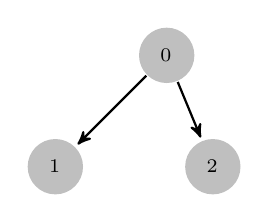
\begin{tikzpicture}[-,>=stealth',shorten >=1pt,auto,node distance=2cm,
			thick]

		\node[vertex] (1) {$\evs_0$};
		\node[vertex] (2) [below left of=1] {$\evs_1$};
		\node[vertex] (3) [right of=2] {$\evs_2$};
		\path[edge]
					(1) edge node {} (2)
					(1) edge node {} (3);
\end{tikzpicture}
\caption{A very simple model that we our previous methodology constructed.
We can immediately see the concept of a ``root" node and ``leaf" nodes.}
\label{exampleModel}
\end{figure}

However, the models we previously generated are not so sensible under an epistemic interpretation.
Indeed, although we can approximate an epistemic event model and the informative update that it
encodes, our resultant model is not so easily interpreted within the original logical systems we
used.
At present, we can thus approximate any event model, whether it is interpretable under epistemic
logics or not.\\
\\
In order to discuss epistemic logic, we need to first impose more restrictions on what axioms our
models must now abide by.
Within a modal logic context, knowledge has a specific structure which results from the axioms
specified in the axiomatic system.
We will move closer to the mainstream axiomatic systems used in epistemic logic by moving to the
axiomatic system $\AXKFF$.
We define the axiomatic system of $\AXKFF$ as follows

\begin{lemma} \label{axiomK45}
The axiomatisation $\AXKFF$ contains the axioms and rules from $\AXK$ (Definition
    \ref{axiomK}), as well as the following axioms
\begin{alignat*}{2}
  & \axFo && \quad \Box \phi \Rightarrow \Box \Box \phi \\
  & \axFi && \quad \Diamond \phi \Rightarrow \Box \Diamond \phi
\end{alignat*}
\end{lemma}

\begin{lemma} \label{axiomK45SoundComplete}
The axiomatisation $\AXKFF$ is sound and complete with respect to the logic
$\lang$.
\end{lemma}

$\AXKFF$ was first constructed by \FIXME and proved to be a sound and complete axiomatic
system by Grossi in \cite{grossi2007designing}.\\
\\
The impact these axioms have on our models is not immediately obvious.
We observe the following effects of the axioms
\begin{itemize}
	\item $\axFo$ causes every relation to be transitive
	\item $\axFi$ has more subtle consequences.
    Suppose $A$ is related to $B$.
    Then if $C$ is related to $A$, $C$ must also be related to $B$.
    A further consequence is that $B$ must also be related to $C$.
\end{itemize}

We demonstrate this in Figure \ref{k45VsKModels} by comparing models in $\AXK$ and $\AXKFF$ and how we need to change
our models to obey these axioms.

\begin{figure}[ht!]
\centering
\begin{subfigure}[b]{.45\textwidth}
\centering
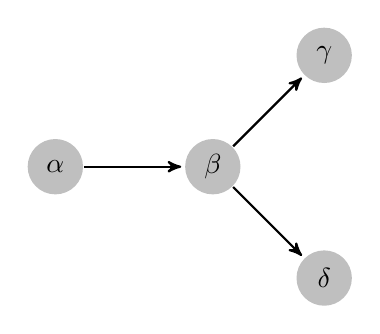
\begin{tikzpicture}[->,>=stealth',shorten >=1pt,auto,node distance=2cm,
      thick]

    \node[vertex] (1) {$\alpha$};
    \node[vertex] (2) [right of=1] {$\beta$};
    \node[vertex] (3) [above right of=2] {$\gamma$};
    \node[vertex] (4) [below right of=2] {$\delta$};
    \path[edge]
          (1) edge node {} (2)
          (2) edge node {} (3)
          (2) edge node {} (4);
\end{tikzpicture}
\caption{Suppose for our Kripke model $\krMo$ (which obeys the rules and axioms in $\AXK$)
  that $\krMo_\alpha \models p$, $\krMo_\beta \models q$, $\krMo_\gamma \models r$ and
  $\krMo_\delta \models q \land p$.
We can say that $\krMo_\alpha \models \Box q$, but we cannot say that $\krMo_\alpha
\models \Box \Box q$.
Then $\axFo$ is disobeyed and thus $\krMo$ is not a $\AXKFF$ event model.}
\label{kmodel}
\end{subfigure}
~
\begin{subfigure}[b]{.45\textwidth}
\centering
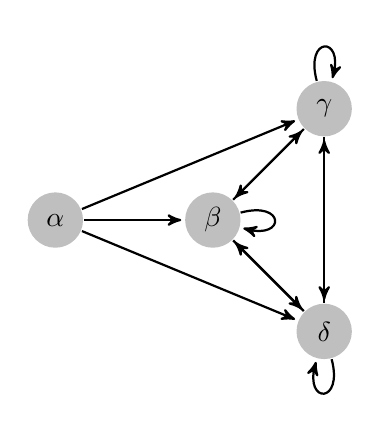
\begin{tikzpicture}[->,>=stealth',shorten >=1pt,auto,node distance=2cm,
      thick]

    \node[vertex] (1) {$\alpha$};
    \node[vertex] (2) [right of=1] {$\beta$};
    \node[vertex] (3) [above right of=2] {$\gamma$};
    \node[vertex] (4) [below right of=2] {$\delta$};
    \path[edge]
          (1) edge node {} (2)
              edge node {} (3)
              edge node {} (4)
          (2) edge node {} (3)
              edge node {} (4)
              edge [loop right] node {} (2)
          (3) edge node {} (2)
              edge node {} (4)
              edge [loop above] node {} (3)
          (4) edge node {} (2)
              edge node {} (3)
              edge [loop below] node {} (4);
\end{tikzpicture}
\caption{Now our Kripke model $\krMo'$ obeys $\AXKFF$.
Let $\krMo'_\alpha \models p, \krMo'_\beta \models q, \krMo'_\gamma \models q \land r$ and
  $\krMo'_\delta) \models q \land p$.
Here, we see that (by $\axFo$) in order to say $\krMo'_\alpha \models \Box q$, we must also be
able to say $\krMo'_\alpha \models \Box \Box q$.}
\label{k45model}
\end{subfigure}
\caption{We compare two Kripke models, $\krMo$ (Subfigure \ref{kmodel}) and
  $\krMo'$ (Subfigure \ref{k45model}).}
\label{k45VsKModels}
\end{figure}

In Figure \ref{k45VsKModels} we compare a Kripke model in $\AXK$ to a model in $\AXKFF$.
We have already briefly discussed how $\axFo$ affects the reasonings we can make on the $\krMo_\alpha$ versus
$\krMo'_\alpha$.
Another observation we can make is with regards to the effect of $\axFi$ on $\krMo'_\alpha$ (Subfigure
\ref{k45model}).
By $\axFi$ for any formula $k \in \lang$ such that $\krMo'_\alpha \models
\Diamond k$, we have that $\krMo'_\alpha \models \Box \Diamond k$.
This causes points $\beta, \gamma$ and $\delta$ to become a completely connected component,
with an edge running to each one of them, as well as reflexive edges for each point.\\
\\
Up to now, what we have shown is an already well-defined idea for whether a Kripke model obeys the axioms of $\AXKFF$.
Unfortunately, this does not translate well to event models due to the differences in their
semantics.
In order to determine if an event model obeys the axioms of $\AXKFF$, we will formalise the ``model"
implications we previously discussed into conditions on the structure of the model (that is, the
frame of the model --- see Definition \ref{frame}).
These are the frame conditions of $\AXKFF$, and we will show that an event model that fulfills these
frame conditions, when executed on a Kripke model that obeys the axioms of $\AXKFF$ will preserve
these axioms post execution.

\begin{lemma} \label{lemma:k45frameconditions}
	Let $F = (S,R)$ be a frame.
	We say that $F$ is a $\AXKFF$ frame if it fulfills the following conditions:
	\begin{itemize}
		\item if $R$ is a transitive relation, then $\axFo$ is valid in any model where $F$ is its
			underlying structure --- that is, for $s, t, u \in S$ then $s R t \land t R u \implies s R u$
		\item if $R$ is a Euclidean relation, then $\axFi$ is valid in any model where $F$ is its
			underlying structure --- that is, for $s, t, u \in S$ then $s R t \land s R u \implies t R u$
	\end{itemize}
\end{lemma}

This is given as an exercise in \cite{fagin1995reasoning}, and we leave it as an exercise to the
reader to show that this holds.
We can use the concept of an $\AXKFF$ frame to define a $\AXKFF$ event model.

\begin{defn} \label{defn:k45eventModel}
	Suppose $\evM = (\evS, \evR, \evpr)$ is an event model.
	We say that $\evM$ is a {\em $\AXKFF$ event model} if $F = (\evS, \evR)$ is a $\AXKFF$ frame.
\end{defn}

The usefulness of a {\em $\AXKFF$ event model} is twofold.
Firstly, it is a structure which has some correspondence to the axioms of $\AXKFF$.
This means it has some epistemic meaning and can be interpreted in a setting that resembles
reasonings about knowledge and belief.
Secondly, we can show that if $\evM_\evT$ is a $\AXKFF$ event model then it preserves the axioms of
$\AXKFF$.

\begin{lemma} \label{lemma:k45preserved}
	Let $\krMo_T = ((S,R,V),T)$ is a $\AXKFF$ Kripke model and $\evM_\evT = ((\evS,\evR,\evpr),\evT)$ is a $\AXKFF$ event model, then
	$\krMo_T \otimes \evM_\evT$ is a $\AXKFF$ Kripke model.
\end{lemma}
\begin{proof}
	Let $\krMo'_{T'} = \krMo_T \otimes \evM_\evT = ((S',R',V'),T')$.\\
	\\
	The first property that will be shown to hold is that $R'$ is a transitive relation.
	Suppose that $s',t',u' \in S'$ such that $s' R'_a t'$ and $t' R'_a u'$.
	From Definition \ref{evModelEx}, $s' = (s,\evs), t' = (t,\evt)$ and $u' = (u,\evu)$ for $s,t,u \in
	S$ and $\evs,\evt,\evu \in \evS$, such that $V(s) \Rightarrow \evpr(\evs)$, $V(t) \Rightarrow
	\evpr(\evt)$ and $V(u) \Rightarrow \evpr(\evu)$.
	Furthermore, $s' R'_a t' \Rightarrow s R_a t \land \evs \evR_a \evt$, and $t' R'_a u' \Rightarrow
	t R_a u \land \evt \evR_a \evu$.
	From $s R_a t \land t R_a u$ we have $s R_a u$, since $R_a$ is a transitive relation by the
	hypothesis.
	Similarly, $\evs \evR_a \evt \land \evt \evR_a \evu \Rightarrow \evs \evR_a \evu$ since $\evR_a$
	is also a transitive relation.
	From Definition \ref{evModelEx}, $s R_a u \land \evs \evR_a \evu \implies (s,\evs) R'_a (u,\evu)
	\Rightarrow s' R'_a u'$.
	Then $R'$ is a transitive relation.\\
	\\
	Similarly we can show that $R'$ is an Euclidean relation.
	Suppose that $s',t',u' \in S'$ such that $s' R'_a t'$ and $s' R'_a u'$.
	From Definition \ref{evModelEx}, $s' = (s,\evs), t' = (t,\evt)$ and $u' = (u,\evu)$ for $s,t,u \in
	S$ and $\evs,\evt,\evu \in \evS$, such that $V(s) \Rightarrow \evpr(\evs)$, $V(t) \Rightarrow
	\evpr(\evt)$ and $V(u) \Rightarrow \evpr(\evu)$.
	Furthermore, $s' R'_a t' \Rightarrow s R_a t \land \evs \evR_a \evt$, and $s' R'_a u' \Rightarrow
	s R_a u \land \evs \evR_a \evu$.
	From $s R_a t \land s R_a u$ we have $t R_a u$, since $R_a$ is an Euclidean relation by the
	hypothesis.
	Similarly, $\evs \evR_a \evt \land \evs \evR_a \evu \Rightarrow \evt \evR_a \evu$ since $\evR_a$
	is also an Euclidean relation.
	From Definition \ref{evModelEx}, $t R_a u \land \evt \evR_a \evu \implies (t,\evt) R'_a (u,\evu)
	\Rightarrow t' R'_a u'$.
	Then $R'$ is an Euclidean relation.\\
	\\
	Since the frame conditions on $(S',R')$ hold $\krMo'_{T'}$ is a $\AXKFF$ Kripke model.
\end{proof}

This shows us that what we consider a $\AXKFF$ event model behaves as we expect --- if we execute
its update on a $\AXKFF$ Kripke model, the resulting Kripke model is also a $\AXKFF$ Kripke model.\\
\\
We can approximate informative updates using our previous method (detailed in Chapter
\ref{chapter:Multiagent}, but these updates do not preserve
axioms $\axFo$ and $\axFi$.
The resulting model barely resembles an epistemic model.
The approach in this chapter constructs event models that, after their execution on a model that
fulfills the conditions of $\AXKFF$, will preserve those conditions.\\
\\
An open question, related to our previous chapter --- can we now generate $\AXKFF$ models to
approximate other $\AXKFF$ models?
\FIXME this paragraph is unclear.

\subsection{Technical Preliminaries --- fixed by 11 September 2013}

We first define what a $B$-insane set is.
It is a necessary condition in order to generate our approximating $\AXKFF$ models.

\begin{defn} \label{binsane}
	Let $\evM_\evT = ((\evS, \evR, \evpre), \evT)$ be a multi-pointed event model and $B \subseteq A$.
	We say that $\evM_\evT$ is {\em $B$-insane} if and only if for all $\evs \in \evT$,
	for all $b \in B$ we have that $\evs \evR_b = \evR_b \evs = \varnothing$.
\end{defn}

If $B = \{b\}$, we say that the set $\evM_\evT$ is $b$-insane.
Similarly if $B = A$ we say that $\evM_\evT$ is simply insane, which fulfills
our previous definition of insanity models (Definition \ref{insanity}).\\
\\
What does it mean for a set of states to be $B$-insane?
If $\evM_\evT$ is $B$-insane, then any agent $b$ in $B$ can distinguish between
action points, but only knows the preconditions of each action point.
They do not actually have any knowledge about what they know or any
introspection at each action point.
This is demonstrated in Figure \ref{bInsaneExample}.
\FIXME might need a pagebreak here.

\begin{figure}[ht!]
\centering
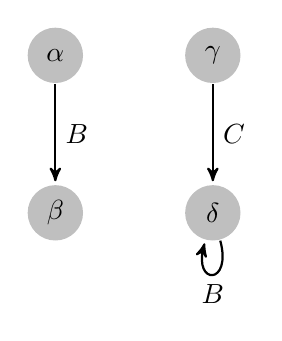
\begin{tikzpicture}[->,>=stealth',shorten >=1pt,auto,node distance=2cm,
      thick]

    \node[vertex] (1) {$\alpha$};
    \node[vertex] (2) [below of=1] {$\beta$};
    \node[vertex] (3) [right of=1] {$\gamma$};
    \node[vertex] (4) [below of=3] {$\delta$};
    \path[edge]
          (1) edge node {$B$} (2)
          (3) edge node {$C$} (4)
          (4) edge [loop below] node {$B$} (4);
\end{tikzpicture}
\caption{Consider our event model $\evM$. Let $B$ and $C$ be mutually exclusive
  subsets of $A$. Here, $\evM_\gamma$
  is $B$-insane, since there are no outgoing or incoming $B$-edges from these event points.
This is easily contrasted with $\evM_\alpha$, which has an outgoing $B$-edge, $\evM_\beta$, which
has an incoming $B$-edge, and $\evM_\delta$ which has a reflexive $B$-edge.}
\label{bInsaneExample}
\end{figure}

We now define the main operation to construct event models in $\AXKFF$ for the
purposes of realising a post condition.

\begin{defn} \label{makeEquivalence}
	Let $B \subseteq A$ and $\evM_\evT$ be a multi-pointed $B$-insane event model.
  For each $\evt \in \evT$ let $\evM_\evt$ be a tree event model in $\AXKFF$.
  Then the operation $I_B(\evM_\evT)$ constructs the event model $\evM'_{\evT'} =
  ((\evS',\evR',\evpr'),\evT')$ such that
  \begin{itemize}
    \item $\evS' = \evS$
    \item $\evR'_a = \evR_a$ if $a \notin B$
    \item $\evR'_a = \evR_a \cup \{(\evs, \evt) | \evs, \evt \in \evT\}$ if $a
    \in B$
    \item $\evpr' = \evpr$
    \item $\evT' = \evT$
  \end{itemize}
\end{defn}

We will say that $I_B$ is an operation that makes all the action
points in a ``distinguished" set of a multi-pointed event model ``equivalent" to a
group of agents $B$.
That is, any agent in $B$ considers each action point $\evs \in \evT$ to be the
same.

\begin{figure}[ht!]
\centering
\begin{subfigure}[b]{.45\textwidth}
\centering
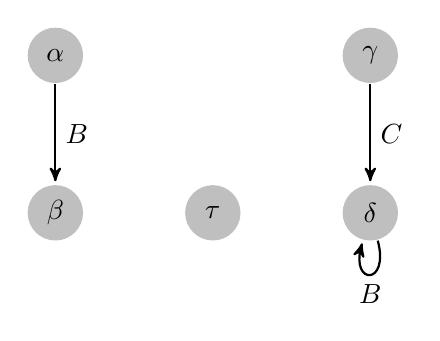
\begin{tikzpicture}[->,>=stealth',shorten >=1pt,auto,node distance=2cm,
      thick]

    \node[vertex] (1) {$\alpha$};
    \node[vertex] (2) [below of=1] {$\beta$};
		\node[vertex] (5) [right of=2] {$\tau$};
    \node[vertex] (4) [right of=5] {$\delta$};
    \node[vertex] (3) [above of=4] {$\gamma$};
    \path[edge]
          (1) edge node {$B$} (2)
          (3) edge node {$C$} (4)
          (4) edge [loop below] node {$B$} (4);
\end{tikzpicture}
\caption{Consider the model $\evMo_\evT$, with $\evT = \{\tau, \gamma\}$.}
\label{beforeOperation}
\end{subfigure}
~
\begin{subfigure}[b]{.45\textwidth}
\centering
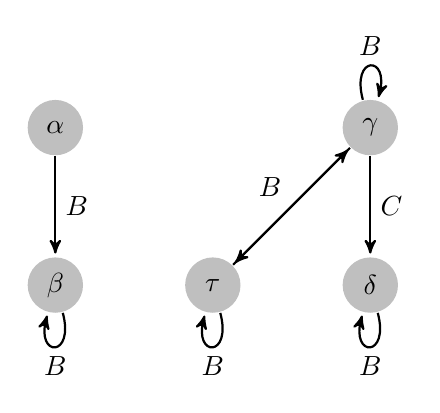
\begin{tikzpicture}[->,>=stealth',shorten >=1pt,auto,node distance=2cm,
      thick]

    \node[vertex] (1) {$\alpha$};
    \node[vertex] (2) [below of=1] {$\beta$};
		\node[vertex] (5) [right of=2] {$\tau$};
    \node[vertex] (4) [right of=5] {$\delta$};
    \node[vertex] (3) [above of=4] {$\gamma$};
    \path[edge]
          (1) edge node {$B$} (2)
					(2) edge [loop below] node {$B$} (2)
					(5) edge [loop below] node {$B$} (5)
							edge node {$B$} (3)
          (3) edge node {$C$} (4)
							edge [loop above] node {$B$} (3)
							edge node {} (5)
          (4) edge [loop below] node {$B$} (4);
\end{tikzpicture}
\caption{Consider our new model $I_B(\evMo_\evT)$, with $\evMo_\evT$ defined as in Subfigure
\ref{beforeOperation}.}
\label{afterOperation}
\end{subfigure}
\caption{Subfigures \ref{beforeOperation} and \ref{afterOperation} demonstrate the effect of
applying our operation $I_B$ onto a model.
Note the }
\label{k45VsKModels}
\end{figure}

In order for us to use our previous operations in $\AXKFF$ we need to force further constraints on
some of our operators.
It is clear that $\sqcup$ will preserve the frame conditions of $\AXKFF$, but $\to_B$ does not.
We will redefine $\to_B$ to ensure that within our language it cannot create event models that are
are not $\AXKFF$ event models.

\begin{defn} \label{defn:k45:considers}
	Suppose $B \subseteq A$ is a subset of agents.
	Let $\evM_\evT = ((\evS,\evR,\evpr),\evT)$ and $\evM'_{\evT'} = ((\evS',\evR',\evpr'),\evT')$ be $\AXKFF$ event models.
	Furthermore, $\evM_\evT$ is a $B$-insane event model, and $\evM'_{\evT'}$ is defined such that for
	all $b$ in $B$, for all $\evt \in \evT'$, $\evt \evR'_b subseteq \evT'$.
	$\evM_\evT \to_B \evM'_{\evT'}$ is defined as in Definition \ref{considers}.
\end{defn}

Note the constraints we place on $\evM_\evT$ and $\evM'_{\evT'}$ being $B$-insane models.
These are necessary in order to preserve the frame conditions in Lemma
\ref{lemma:k45frameconditions}.

\newcommand{\EM}{\ensuremath{\eventClass}}

The addition of our new operator results in us having the following language for
event model construction in $\AXKFF$.
\[
	\evM_\evT ::= \aMod{M_s} \text{ } | \text{ }\evM_\evT \to_B \evM'_{\evT'} \text{ }|
  \text{ } \evM_\evT \sqcup \evM'_{\evT'} \text{ } | \text{ } I_B(\evM_\evT)
\]
where $\aMod{M_s} \in \insaneClass, \evM_\evT, \evM'_{\evT'}$ are multi-pointed event models and $B \subseteq
A$ is a subset of agents.
We will refer to our language as $\EM(\to,\sqcup,I)$. \\
\\
We will now show that this language always constructs models that preserve $\AXKFF$, and that any
event model that preserves the axioms of $\AXKFF$ can be constructed by our language.

\subsection{Some Interesting Technical Results}

To show that we can construct event models that preserve $\AXKFF$, there are two propositions that
must hold
\begin{enumerate}
	\item we can use our language to construct event models that will preserve $\AXKFF$
	\item an event model that preserves $\AXKFF$ can be constructed (up to $n$-bisimilarity) by our
		language
\end{enumerate}

Let us show that the first proposition --- that $\EM(\to,\sqcup,I)$ will construct $\AXKFF$ event
models.

\begin{lemma}
	Let $\evM_\evT$ be a pointed event model constructed from the language $\EM(\to,\sqcup,I)$.
	Then $\evM_\evT$ is a $\AXKFF$ event model.
\end{lemma}
\begin{proof}
	We can show this through a case-by-case proof that each of the operations and atoms using in
	$\EM(\to,\sqcup,I)$ constructs a $\AXKFF$ event model.
	We first examine the atoms using in $\EM(\to,\sqcup,I)$ and show that they are $\AXKFF$ event
	models.\\
	\\
	Since the only atomic event models we use in $\EM(\to,\sqcup,I)$ are insanity models, we suppose
	that $\evM_{\evt} = ((\evS,\evR,\evpr),\{\evt\})$, where $\evS = \{\evt\}$ and $\evR =
	\varnothing$.
	This is a $\AXKFF$ frame since $\evR = \varnothing$ ensures that the frame conditions
	are trivially true.\\
	\\
	We now will show that $\sqcup$ constructs $\AXKFF$ event models.
	Let $\evM_\evT = ((\evS,\evR,\evpr),\evT)$ and $\evM'_{\evT'} = ((\evS',\evR',\evpr'),\evT')$ be
	$\AXKFF$ event models such that $\evS$ and $\evS'$ are disjoint.
	Now, let $\evM''_{\evT''} = \evM_\evT \sqcup \evM'_{\evT'} = ((\evS'',\evR'',\evpr''),\evT'')$.
	We need to show that the two frame conditions outlined in Lemma \ref{lemma:k45frameconditions}
	hold.\\
	\\
	We will show the first frame condition --- that is, that $\evR''$ is a transitive relation.
	Suupose that for $a \in A$ and $\evs'', \evt'', \evu'' \in \evS''$ such that $\evs'' \evR''_a
	\evt''$ and $\evt'' \evR''_a \evu''$, we must show that $\evs'' \evR''_a \evu''$.
	We have from Definition \ref{disjoint} that $\evR'' = \evR \sqcup \evR'$, $\evS'' = \evS \sqcup
	\evS'$ and from hypothesis that both $\evS$ and $\evS'$ are disjoint.
	We observe that from Definition \ref{disjoint}, the operation $\sqcup$ will construct no new
	relations from any element in $\evS$ to an element in $\evS'$ and vice versa.\\
	\\
	Then $\evs'', \evt'', \evu''$ must all originally be elements of either $\evS$ or $\evS'$ ---
	without loss of generality, we say that they are elements of $\evS$.
	Furthermore, then relation $\evs'' \evR''_a \evt''$ and $\evt'' \evR''_a \evu''$ also correspond
	to $\evs'' \evR_a \evt''$ and $\evt'' \evR_a \evu''$.
	Since $\evM_\evT$ is a $\AXKFF$ event model, then $\evs'' \evR_a \evt''$ and $\evt'' \evR_a \evu''$
	yields that $\evs'' \evR_a \evu''$, which implies that $\evs'' \evR''_a \evu''$.
	This shows that the transitivity frame condition holds.
	A similar argument can be made to show that $\evR''$ is a Euclidean relation.
	Thus, we have shown that $\evM''_{\evT''} = \evM_\evT \sqcup \evM'_{\evT'}$ is a $\AXKFF$ event
	model.\\
	\\
	We next show that $I_B$ is an $\AXKFF$ event model.
	Suppose that $\evM_\evT$ is a $B$-insane $\AXKFF$ event model.
	We will show that $\evM'_{\evT'} = ((\evS',\evR',\evpr'),\evT') = I_B(\evM_\evT)$ is an $\AXKFF$ event model, by showing the frame conditions in
	Lemma \ref{lemma:k45frameconditions}.\\
	\\
	Let us show that $\evR'$ is a transitive relation.
	Suppose that $a \in A$ and $\evs', \evt', \evu' \in \evS'$ and $\evs' \evR'_a \evt'$ and $\evt'
	\evR'_a \evu'$.
	We must show that $\evs' \evR'_a \evu'$.
	We note that this condition is already true if $a \notin B$ or $

\end{proof}

We have shown that any event models generated from $\EM(\to,\sqcup, I)$ are
$\AXKFF$ event models.
Thus, we can guarantee that if $\evM_\evT$ is a model generated by
$\EM(\to,\sqcup,I)$ and $\krMo_T$ is a $\AXKFF$ Kripke model, $\krMo_T
\otimes \evM_\evT$ is also a $\AXKFF$ Kripke model.
This shows that the constructions we use --- $\EM(\to, \sqcup, I)$ are
sound, and will preserve the axioms of $\AXKFF$ after their execution.\\
\\
Let us turn to the second goal we have and suppose that we have an event model, $\evM_\evT
= ((\evS,\evR,\evpr),\evT)$ that is a $\AXKFF$ multi-pointed event model.
Now, consider $n$ some positive integer.
Can we construct an event model $\evM'_{\evT'} = ((\evS',\evR',\evpr'),\evT')$
using $\EM(\to,\sqcup,I)$ that is $n$-bisimilar to $\evM_\evT$?

In order to show this to be possible, we must first conceptualise several
transformations to our models.
Firstly, we will define the idea of an unwound model.

\begin{defn}\label{def:unwoundModel}
  Suppose $\evM_\evT = ((\evS,\evR,\evpr),\evT)$ is a $\AXKFF$ multi-pointed
  event model.
  There is an event model, $\evM'_{\evT'} = ((\evS',\evR',\evpr'),\evT')$ such that
  \begin{itemize}
		\item $\evS'$ is the set of words $\evs \evS^\ast$, where $\evs \in \evT'$
			\footnote{We can consider each action point $\evs$ in the model to be labelled with the string of
			points it took to go from an element $\evt \in \evT'$ to $\evs$.
			Then $\evS^\ast$ is the set of strings (including $\lambda$, the empty word) over the alphabet 
			of $\evS$.}
		\item $\evR'_a$ is the transitive Euclidean closure of the set of relations $\{(\evp \evt,
			\evp \evt \evu)$ where $\evp \in \evS^\ast$ and $\evt \evR_a \evu$, for $\evt, \evu \in \evS \}$
		\item $\evpr'(\evp \evt) = \evpr(\evt)$
		\item $\evT' = \evT$
  \end{itemize}
  We say that $\evM'_{\evT'}$ is the {\em unwound model} of $\evM_\evT$.
\end{defn}

\begin{lemma} \label{lemma:unwoundModel:bisimilar}
  Suppose $\evM_\evT = ((\evS,\evR,\evpr),\evT)$ is a $\AXKFF$ multi-pointed
  event model.
	Let $\evM'_{\evT'} = ((\evS',\evR',\evpr'),\evT')$ be the unwound model of $\evM_\evT$.
	Then $\evM'_{\evT'}$ is a $\AXKFF$ event model and $\evM'_{\evT'} \sim \evM_\evT$.
\end{lemma}
\begin{proof}
	By the definition of an unwound model, we can see that the frame conditions in Lemma 
	\ref{lemma:k45frameconditions} will automatically be fulfilled.\\
	\\
	It remains to be shown that $\evM'_{\evT'} \sim \evM_\evT$.
	We define $\sim$ as
	\[
		\{(\evs',\evs) \text{ such that } \evs' \in \evS \land \evs \in \evS \land \evs' = \evp \evs
			\text{ where } \evp \in \evS^\ast \land \evpr'(\evs') \iff \evpr(\evs) \}
	\]

	From our definition of $\sim$, we have that $\evs' \sim \evs \iff (\evpr'(\evs') \iff
	\evpr(\evs))$.
	We now must check {\bf forth-$a$} and {\bf back-$a$}.\\
	\\
	Let $a \in A$ and $\evs' \in \evS' \land \evs' \evR'_a \evt'$.
	Suppose $\evs' \sim \evs \in \evS$.
	By the definition of $\sim$, $\evs' = \evp \evs$ where $\evp \in \evS^\ast$.
	From the definition of an unwound model, $\evt' = \evp \evs \evt$, where $\evt$ is some action
	point such that $\evs \evR_a \evt$.
	Since $\evs' \in \evS^\ast$, and we have $\evt' = \evs' \evt$ then $\evt' \sim \evt$.
	Then {\bf forth-$a$} holds.
	A similar proof can be shown for {\bf back-$a$}.
	Since both of these hold, we can say that $\evM'_{\evT'} \sim \evM_\evT$.
\end{proof}

The unwound model is an infinite pseudo-forest event model.
This means that the model somewhat resembles our original forest event models,
but with interior relations between the action points, and without the
restriction of finiteness.
We show an example of this in Figure \ref{generatedTreeExample}

\begin{figure}[ht!]
\centering
\caption{\FIXME Left subfigure should be original, right subfigure should be the
unwound model.} \label{generatedTreeExample}
\end{figure}

The unwound model is bisimilar to the original $\AXKFF$ event model.
However, as it may be an infinite event model (in terms of the number of action
points), it is undesirable to try and construct this model.
Furthermore, most of the time, we might only be interested in the
post-conditions of a event model that are up to some modal depth.
If we instead consider a finite submodel of the unwound model
model, we can show that this submodel is $n$-bisimilar to $\evM_\evT$.

\begin{defn} \label{unwoundNModel}
  Suppose $\evM_\evT = ((\evS,\evR,\evpr),\evT)$ is a $\AXKFF$ multi-pointed event model, and
	let $\evM''_{\evT''} = ((\evS'',\evR'',\evpr''),\evT'')$ be the unwound model of $\evM_\evT$.
  Let $n$ be some positive integer and let $\evM'_{\evT'} = ((\evS',\evR',\evpr'),\evT')$ be an event model such that
  \begin{itemize}
		\item $\evS' = \evs \evp$, where $\evp \in \evS^\ast$ is a string of length
    less than $n$ and $\evs \in \evT$
		\item $\evR'$ is $\evR''$ restricted to $\evS'$
		\item $\evpr'$ is $\evpr''$ restricted to $\evS'$
		\item $\evT' = \evT''$
  \end{itemize}
  We say that $\evM'_{\evT'}$ is the {\em unwound $n$-model} of $\evM_\evT$.
\end{defn}

\begin{lemma} \label{lemma:unwoundNModelNBisimilar}
  Suppose $\evM_\evT = ((\evS,\evR,\evpr),\evT)$ is a $\AXKFF$ multi-pointed
  event model.
  Let $n$ be some positive integer and $\evM''_{\evT''} = ((\evS'',\evR'',\evpr''),\evT'')$ be the
	unwound $n$-model of $\evM_\evT$.
  Then $\evM_\evT \sim_n \evM''_{\evT''}$.
\end{lemma}
\begin{proof}
	We will induct over $n$ to show that this holds.
	We hypothesise that for every action point $\evt \in \evT''$, $\evM''_\evt \sim_k \evM'_{\evt}$
	for some $0 \leq k \leq n$.\\
	\\
	We begin with our base case of $k = 0$.
	Since $\evT' = \evT''$ then $\evt \in \evT'' \Rightarrow \evt \in \evT'$.
	It is clear that $\evt$ is $0$-bisimilar to itself, and therefore we conclude that $\evM''_\evt
	\sim_0 \evM'_\evt$.\\
	\\
	Now, suppose that for $k = m$, our hypothesis holds.\\
	\\
	We will show that it now holds for $k = m+1$.
	We have already shown that $\evM''_\evt \sim_{k-1} \evM'_\evt$, through the inductive step.
	We must now show both of {\bf $k$-forth-$a$} and {\bf $k$-back-$a$} as in Definition
	\ref{nBisimEvent}.\\
	\\
	Let us show {\bf $k$-forth-$a$}.
	Let $a \in A$, and suppose that $\evs \in \evt \evR''_a$.
	We want to show there is some $\evs' \in \evt \evR'_a$ such that $\evs' \sim_{k-1} \evs$.
	To show that this is so, we would require that $\evs' \sim_{k-2} \evs$, and that {\bf
	$k-1$-forth-$a$} and {\bf $k-1$-back-$a$} both hold at $\evs$.\\
	\\
	We can continue this argument until we reach some new point $\evs \in \evS''$ that we require to be
	$0$-bisimilar to some other point $\evs' \in \evS'$.
	It is clear that these new points are 0-bisimilar, that is $\evs \sim_0 \evs'$, which allows us to
	claim that {\bf $k$-forth-$a$} is originally satisfied at $\evt$.\\
	\\
	We can make a similar argument for {\bf $k$-back-$a$} and through this we can satisfy the
	conditions of Definition \ref{nBisimEvent}, allowing us to claim that for all $\evM''_\evt \sim_k
	\evM'_{\evt}$.
\end{proof}

This submodel of the unwound model is $n$-bisimilar to our original $\evM_\evT$
and is finite, which are both desirable properties.
Using our previous example, we show in Figure \ref{genSubtreeExample} the
finite submodel that is $n$-bisimilar.

\begin{figure}[ht!]
\centering
\caption{\FIXME Show finite version of figure \ref{generatedTreeExample}} \label{genSubtreeExample}
\end{figure}

It remains to be shown that we can actually construct an unwound $n$-model using
$\EM(\to,\sqcup,I)$.
We will now show that we can actually construct any unwound $n$-model using $\EM(\to,
\sqcup, I)$, up to $n$-bisimilarity.

\begin{lemma} \label{lemma:unwoundModelBisimilarConstruct}
  Suppose $\evM_\evT = ((\evS,\evR,\evpr),\evT)$ is a $\AXKFF$ multi-pointed
  event model.
	Let $\evM'_{\evT'} = ((\evS',\evR',\evpr'),\evT')$ be the unwound model of
  $\evM_\evT$ and $n$ be some non-negative integer.
  We can construct an event model using $\EM(\to,\sqcup,I)$ that is $n$-bisimilar to
  $\evM'_{\evT'}$.
\end{lemma}
\begin{proof}
	Consider $\evs' \in \evS'$, where $\evs' = \evp \evs$ for some $\evp \in \evS^\ast$ and $\evs \in
	\evS$, and $0 \leq k \leq n$.
	We will consider a submodel of $\evM'_{\evT'}$, $\evM^k_{\evs'} =
	((\evS^k,\evR^k,\evpr^k),\{\evs'\})$, such that
	\begin{itemize}
		\item $\evS^k = \evs' \evp$, where $\evp \in \evS^\ast$ and $\evp$ is a string of length less
			than $k$
		\item $\evR^k_a = \evR'$ restricted to $\evS^k$ if $\evR'_a \evs'$ is empty
		\item $\evR^k_a = \evR' \setminus \{\evs' \evR^k_a = \evR^k_a \evs'\}$,
    restricted to $\evS^k$ if $\evR'_a \evs$ is nonempty
		\item $\evpr^k = \evpr'$ restricted to $\evS^k$
	\end{itemize}

	It is clear that when $\evs' \in \evT'$, there is no $\evt' \in \evS'$ such
  that for $a \in A$, $\evt' \evR'_a \evs'$.
  Then $\evM^k_{\evs'}$ is the unwound $k$-model of $\evM_\evs$.
	It will thus be sufficient to use this representation of a subtree and show that we can construct
	some event model that is bisimilar to $\evM'_\evs$.\\
	\\
	To show this we will induct over $k$, from 0 to $n$.
	Our induction hypothesis is as follows.
  For any point $\evs' \in \evS'$ we can construct a model using
  $\EM(\to,\sqcup,I)$, $\evM^{k'}_{\evs''}$ that is bisimilar to $\evM^k_{\evs'}$.\\
	\\
	Let $k = 0$.
	Let $\evM^{0'}_{\evs''} = ((\evS^{0'},\evR^{0'},\evpr^{0'}),\{\evs'\}) \in \insaneClass$ where
	\begin{itemize}
		\item $\evS^{0'} = \{\evs''\}$
		\item $\evR^{0'} = \varnothing$
		\item $\evpr^{0'} = \{(\evs'',\evpr(\evs))\}$
	\end{itemize}

	As $\evpr^{0'}(\evs'') = \evpr(\evs) = \evpr'(\evs')$ then $\evpr^{0'}(\evs'') \iff
  \evpr'(\evs')$.
	Then $\evM^{0'}_{\evs'} \sim \evM^0_{\evs'}$.\\
	\\
	Now, we suppose that the induction hypothesis holds for $k$.
	We will show it also holds for $k+1$.
	We need only consider $a \in A$ such that $\evR'_a \evs'$ is empty.
	We shall call these agents $A' = \{a_1,a_2,\ldots,a_j\}$.
  \\
  Let $a' \in A'$, and $\evs' \evR'_{a'} \evt'$.
  We can construct a model $\evM^{k'}_{\evt''}$ using $\EM(\to,\sqcup,I)$ that is
  bisimilar to $\evM^k_{\evt'}$.
  Since $\evs' \evR'_{a'} \evt'$ then $\evt'' \evR^{k'}_{a'} = \evR^{k'}_{a'}
  \evt'' = \varnothing$.
  Then $\evM^{k'}_{\evt''}$ is $a'$-insane and this holds for every $\evt' \in
  \evs' \evR'_{a'}$.\\
  \\
  Then
  \[
    \bigsqcup_{\evt' \in \evs' \evR'_{a'} \land \evM^{k'}_{\evt''} \sim_k
      \evM^k_\evt} \evM^{k'}_{\evt'}
  \]
  is also an $a'$-insane model (although we have not shown this previously, it
  is quite clear from the definition of $\sqcup$), which allows us to construct the model
  \[
    \evM^{k'}_{\evT^{a'}} = I_{a'}(\bigsqcup_{\evt' \in \evs' \evR'_{a'} \land \evM^{k'}_{\evt''} \sim_k
      \evM^k_\evt} \evM^{k'}_{\evt'}) = ((\evS^{k'},\evR^{k'},\evpr^{k'}),\evT^{a'})
  \]

  It is clear that for $\evt'' \in \evT'$, $\evt'' \evR^{k'}_{a'} = \evT^{a'}$, by the
  definition of $I_{a'}$ and the definition of $\evM^{k'}_{\evt'}$.
  We can form a similar model for each of $a_1,a_2,\ldots,\a_j \in A'$, which is
  $\evM^{k'}_{\evT^{a_1}}, \evM^{k'}_{\evT^{a_2}}, \evM^{k'}_{\evT^{a_3}},
  \ldots, \evM^{k'}_{\evT^{a_j}}$ respectively.
  We now consider the model $\evM^{0'}_{\evs'}$, as defined in our base case,
  which is bisimilar to $\evM^0_{\evs'}$.
  We note that it is trivially $a'$-insane for all $a' \in A'$.\\
  \\
  The two conditions we outlined in the previous paragraph allow us to use the $\to_{a'}$ operation as follows
  \[
    \evM^{k+1'}_{\evs'} = (\ldots((\evM^0_{\evs'} \to_{a_1}
            \evM^{k'}_{\evT^{a_1}}) \to_{a_2} \evM^{k'}_{\evT^{a_2}}) \to_{a_3}
        \ldots ) \to_{a_j} \evM^{k'}$
  \]

  This model is a $\AXKFF$ event model, since the operations used to construct
  it were $\EM(\to,\sqcup,I)$.
  It remains to be shown that $\evM^{k+1'}_{\evs''} \sim \evM^{k+1}_{\evs'}$.\\
  \\
  We will construct the following relation $\sim$ over $\evS^{k+1'} \times
  \evS^{k+1}$ such that $(\evt',\evt) \in \sim \iff \evM^{i'}_{\evt'} \sim
  \evM^{i}_{\evt}$ for some $0 \leq i \leq k$, or $\evt' = \evs'' \land \evt =
  \evs'$.
  We will show that this is a bisimulation.\\
  \\
  We note that for any pair $(\evt',\evt)$, $\evpr^{k+1'}(\evt') \iff
  \evpr^{k+1}(\evt)$ since $\evM^{i'}_{\evt'} \sim \evM^{i}_{\evt}$.
  It remains to be shown that if $(\evt', \evt) \in \sim$ then both {\bf
  forth-$a$} and {\bf back-$a$} hold.  
%  We want to show that forth-$a$ holds
%  If we get a point pairing $(\evt', \evt)$, and
%  lets say that $\evt' \evR^{k+1'}_a \evu'$, then there is a point in $\evu \in
%  \evt \evR^{k+1}$ such that $(\evu',\evu)$.
%  If $\evR^{k+1}_a \evt'$ is empty, then $\evM^{i'}_{\evu'} \sim
%  \evM^i_{\evu}$.

%  \\
%  Let us show that {\bf forth-$a$} holds.
%  Suppose $(\evt', \evt) \in \sim$ and let $a \in A$.
%  Consider the point $\evu' \in \evt' \evR^{k+1'}_a$.
%  We note that $\evt' \evR^{k+1'}_a \evu' \iff \evR^{k+1'}_a \evt' = \varnothing$.
%  We must show that there is some $\evu \in \evt \evR^{k+1}_a$ such that
%  $(\evu',\evu) \in \sim$.
%  \\
%  We note that some submodel of $\evM^{k+1}_{\evs'}$, $\evM^i_{\evt}$ is
%  bisimilar to a submodel of $\evM^{k+1'}_{\evs''}$, which is
%  $\evM^{i'}_{\evt'}$.
%  The relations for $\evt' \evR^{i'}_a$ and $\evt \evR^{i}_a$ are both the empty set, which
%  is different from $\evt' \evR^{k+1'}_a$ and $\evt \evR^{k+1}_a$.
%  This is the only difference between $\evM^{i}_{\evt}$ and
%  $\evM^{k+1}_{\evt}$, and $\evM^{i'}_{\evt'}$ and $\evM^{k+1'}_{\evt'}$.\\
%  \\
%  Due to taking the transitive Euclidean closure of relations in the original unwound
%  model, we have that our construction 
\end{proof}

%\begin{defn} \label{unwoundNModel}
%  Suppose $\evM_\evT = ((\evS,\evR,\evpr),\evT)$ is a $\AXKFF$ multi-pointed event model, and
%	let $\evM''_{\evT''} = ((\evS'',\evR'',\evpr''),\evT'')$ be the unwound model of $\evM_\evT$.
%  Let $n$ be some positive integer and let $\evM'_{\evT'} = ((\evS',\evR',\evpr'),\evT')$ be an event model such that
%  \begin{itemize}
%		\item $\evS' = \evs \evS^{n-1}$ and $\evs \in \evT$
%		\item $\evR'$ is $\evR''$ restricted to $\evS'$
%		\item $\evpr'$ is $\evpr''$ restricted to $\evS'$
%		\item $\evT' = \evT''$
%  \end{itemize}
%  We say that $\evM'_{\evT'}$ is the {\em unwound $n$-model} of $\evM_\evT$.
%\end{defn}
%
%\begin{lemma} \label{lemma:unwoundNModelNBisimilar}
%  Suppose $\evM_\evT = ((\evS,\evR,\evpr),\evT)$ is a $\AXKFF$ multi-pointed
%  event model.
%  Let $n$ be some positive integer and $\evM''_{\evT''} = ((\evS'',\evR'',\evpr''),\evT'')$ be the
%	unwound $n$-model of $\evM_\evT$.
%  Then $\evM_\evT \sim_n \evM''_{\evT''}$.
%\end{lemma}
%\begin{proof}
%	We will induct over $n$ to show that this holds.
%	We hypothesise that for every action point $\evt \in \evT''$, $\evM''_\evt \sim_k \evM'_{\evt}$
%	for some $0 \leq k \leq n$.\\
%	\\
%	We begin with our base case of $k = 0$.
%	Since $\evT' = \evT''$ then $\evt \in \evT'' \Rightarrow \evt \in \evT'$.
%	It is clear that $\evt$ is $0$-bisimilar to itself, and therefore we conclude that $\evM''_\evt
%	\sim_0 \evM'_\evt$.\\
%	\\
%	Now, suppose that for $k = m$, our hypothesis holds.\\
%	\\
%	We will show that it now holds for $k = m+1$.
%	We have already shown that $\evM''_\evt \sim_{k-1} \evM'_\evt$, through the inductive step.
%	We must now show both of {\bf $k$-forth-$a$} and {\bf $k$-back-$a$} as in Definition
%	\ref{nBisimEvent}.\\
%	\\
%	Let us show {\bf $k$-forth-$a$}.
%	Let $a \in A$, and suppose that $\evs \in \evt \evR''_a$.
%	We want to show there is some $\evs' \in \evt \evR'_a$ such that $\evs' \sim_{k-1} \evs$.
%	To show that this is so, we would require that $\evs' \sim_{k-2} \evs$, and that {\bf
%	$k-1$-forth-$a$} and {\bf $k-1$-back-$a$} both hold at $\evs$.\\
%	\\
%	We can continue this argument until we reach some new point $\evs \in \evS''$ that we require to be
%	$0$-bisimilar to some other point $\evs' \in \evS'$.
%	It is clear that these new points are 0-bisimilar, that is $\evs \sim_0 \evs'$, which allows us to
%	claim that {\bf $k$-forth-$a$} is originally satisfied at $\evt$.\\
%	\\
%	We can make a similar argument for {\bf $k$-back-$a$} and through this we can satisfy the
%	conditions of Definition \ref{nBisimEvent}, allowing us to claim that for all $\evM''_\evt \sim_k
%	\evM'_{\evt}$.
%\end{proof}
%
%This submodel of the unwound model is $n$-bisimilar to our original $\evM_\evT$
%and is finite, which are both desirable properties.
%Using our previous example, we show in Figure \ref{genSubtreeExample} the
%finite submodel that is $n$-bisimilar.
%
%\begin{figure}[ht!]
%\centering
%\caption{\FIXME Show finite version of figure \ref{generatedTreeExample}} \label{genSubtreeExample}
%\end{figure}
%
%It remains to be shown that we can actually construct an unwound $n$-model using
%$\EM(\to,\sqcup,I)$.
%We will now show that we can actually construct any unwound $n$-model using $\EM(\to,
%\sqcup, I)$.
%
%\begin{lemma} \label{unwoundNModelGenerated}
%  Suppose $\evM_\evT = ((\evS,\evR,\evpr),\evT)$ is a $\AXKFF$ multi-pointed
%  event model.
%  Let $n$ be some positive integer and let $\evM'_{\evT'} = ((\evS', \evR', \evpr'),\evT')$
%  be the unwound $n$-model of $\evM_\evT$.
%  $\evM'_{\evT'}$ can be constructed by $\EM(\to, \sqcup, I)$, up to $n$-bisimilarity.
%\end{lemma}
%\begin{proof}
%  We will show this holds using a proof by induction over $n$.
%\end{proof}

Using this result, we can now construct, up to $n$-bisimilarity, an
approximation of any update using semantically meaningful operations.
This means that we can approximate any update, with the size of our resulting
model dependent on the depth of the post-conditions we are interested in.
A corollary to this result follows with regards to the single agent case.

\begin{corr}
  Suppose $\evM_\evT = ((\evS,\evR,\evpr),\evT)$ is a $\AXKFF$ multi-pointed
  event model involving only one agent, $a$.
  We can construct $\evM'_{\evT'} = ((\evS',\evR',\evpr'),\evT')$ by
  $\EM(\to,\sqcup,I)$ where $\evM'_{\evT'} \sim \evM_\evT$.
\end{corr}
\begin{proof}
	\FIXME proof, it's not safe to go alone
\end{proof}

\section{Conclusion --- fixed by 14 October 2013}

We have shown methods to construct epistemic event models (that is, epistemic updates) in two different axiom systems --- $\AXK$
and $\AXKFF$.
We have employed a set of meaningful operations in both systems in order to construct event models.
In doing so, we have also shown that if there is an appropriate epistemic goal, then
\begin{itemize}
	\item in $\AXK$ we can construct an event model that will achieve that epistemic goal
	\item in $\AXKFF$, if an update model exists that achieves the epistemic goal, we can construct an
$\AXKFF$ event model that will have also achieve this goal
\end{itemize}

It is important to note that event models, their synthesis, and their practical applications in
developing protocols have not been well examined.
Our work has specified operations that are meaningful in their axiomatic systems, and we have proven
that for some event model $\evM_\evT$ we can use our operations to form event models that will
achieve the same post-conditions as $\evM_\evT$ after execution.
This is a first step in employing event models as updates in knowledge base systems, especially
games, model checking and financial systems.
This is due to our operations provide a high-level, theoretical way to construct updates which we know are correct.
Furthermore, we know that the updates we can construct are complete --- that is, they can achieve
all the same epistemic goals as other updates.\\
\\
We have yet to further explore how succinct our updates are.
Can we make the smallest update?
Can we make update that changes the knowledge base in the ``smallest way"?
Furthermore, even if we can construct so many different kinds of updates, what updates are the most
useful?
Which event models or updates might we be most interested in constructing, and if so are there
better methods of constructing them?\\
\\
The work in this paper outlines an approach to event model construction that is rudimentary, but is,
to the author's knowledge, one of the first steps in an unexplored area.
Event models, as updates for which properties can be both proven and reasoned about, are powerful
constructs.
By having event model construction tools, we have the first steps towards employing event models and
the updates they represent in dynamic automated multiagent systems.

% Every research paper should answer the following questions:
% 
% \begin{itemize}
% \item What did you do?
% \item Why did you do it?
% \item What happened?
% \item What do the results mean?
% \item What is your work good for?
% \end{itemize}
% 
% Make sure that your conclusion leaves the reader with the answers
% to these questions clearly in mind.
% 

\section*{Acknowledgements}

I would like to acknowledge Tim French and James Hales for their valued assistance during this final
year engineering project.

% appendices

\bibliographystyle{ieeetr}
\bibliography{thesis}

\end{document}
